\documentclass[a4paper,cleardoubleempty]{scrreprt}
\usepackage[utf8]{inputenc}
\usepackage{amsmath,amssymb, amsthm, commath}
\usepackage[pdftex,bookmarks=false,pdfpagelabels=true,plainpages=false]{hyperref}
\usepackage{booktabs}
\usepackage{makeidx}
\usepackage{url}
%\usepackage{sfmath}
\usepackage{color}
\usepackage{graphicx} 
\usepackage{enumerate}
\usepackage{listings}

\theoremstyle{plain}
\newtheorem{Problem}{Problem}[section]

\theoremstyle{remark}
\newtheorem{remark}[Problem]{Remark}

%%% Geht bei mir nicht: habe tex neu installiert, geht aber trotzdem nicht
%\usepackage{changes}
%\usepackage{todonotes}

%\newcommand{\twick}[1]{\added{#1}}
%\newcommand{\twickremove}[1]{\deleted{#1}}



\newcommand{\dope}{\texttt{DOpElib}}

\makeindex

%%%%%%%%%%%%%%%%%%%%%%%%%%%%%%%%%%%%%%%%%%%%%%%%%%
\begin{document}
\title{DOpElib:\\ 
Differential Equations and Optimization Environment}
\author{
  Thomas Wick\thanks{École Polytechnique, 
    {thomas.wick@polytechnique.edu}}, 
  Winnifried Wollner\thanks{Technische Universität Darmstadt, 
    {wollner@mathematik.tu-darmstadt.de}}
}




\date{\today
\vspace*{2cm}
\begin{figure}[h]
\centering
{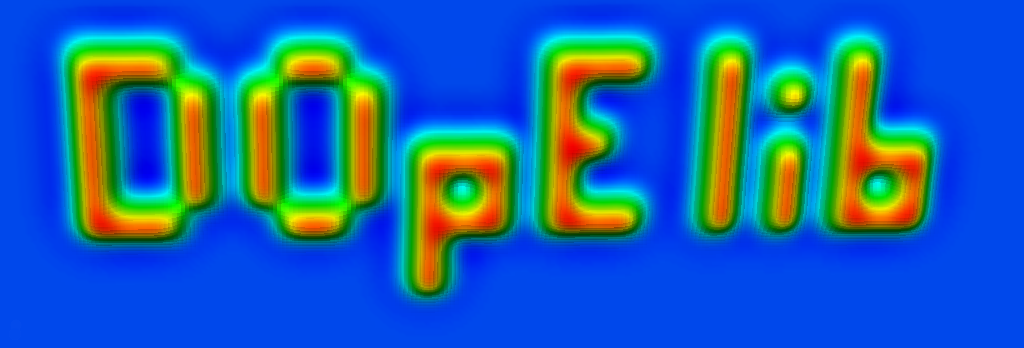
\includegraphics[width=8cm]{Documentation/logo.png}}
\end{figure}
}


%%%%%%%%%%%%%%%%%%%%%%%%%%%%%%%%%%%%%%%%%%%%%%%%%%
\maketitle
\cleardoublepage\pagestyle{headings}
\tableofcontents
\cleardoublepage

%%%%%%%%%%%%%%%%%%%%%%%%%%%%%%%%%%%%%%%%%%%%%%%%%%%
\chapter{Foreword}
\textcolor{red}{Ich habe Section 2.8 etc. 'how this library is structured' zu 
einem eigenen chapter gemacht}
In this report, we describe the \dope{}
\textit{Differential Equations and  Optimization Environment} project. 
Originally, the project was initiated in the year 2009 at the 
University of Heidelberg (Germany) in the numerical analysis
group of Rolf Rannacher. 


\textcolor{blue}{Eigentlich kann dieser ganze paragraph weg. Im naechsten
  Paragraphen steht das
im Prinzip nochmal!
Its key feature is to give a unified interface to high level algorithms such as 
time stepping methods, nonlinear solvers and optimization routines. 
We aim that the user should only need to write those parts
of code that are problem dependent while all invariant parts of the algorithms
should be reusable without any need for further coding.
In particular, the user should be able to switch between various different 
algorithms without the need to rewrite the problem dependent code, though he or she will
have to replace the algorithm object with an other one. 
Another aim of \dope{} is to provide a software toolkit to solve forward PDE
problems as well as optimal control problems constrained by PDE. The
solution of a broad variety of PDE is possible in deal.II as well, but
\dope{} concentrates on a unified approach for both linear and nonlinear
problems by interpreting every PDE problem as nonlinear and applying a
Newton method to solve it. 
The focus is on the numerical solution of both stationary and nonstationary
problems which come from different application fields, like elasticity and
plasticity, fluid dynamics, and multiphysics problems such as 
fluid-structure interactions.
}

The main feature of \dope{} is to give a unified interface to high level 
algorithms such as 
time-stepping methods, nonlinear solvers and optimization routines. 
\dope{} is designed in such a way that the user only needs to write those parts
of the code that are problem dependent while all invariant 
parts of the algorithms
are reusable without any need for further coding.
In particular, the user is enabled to switch between various different 
algorithms without the need to rewrite the problem dependent code, 
though obviously he or she will
have to replace the algorithm object with an other one. 
This replacement can be done by replacing the appropriate object at only
one point in the code.
In addition to the finite element code provided by deal.II --which at present is the only FE-toolkit to which we provide an 
interface-- 
the presented library
\dope{} is user-focused by delivering
prefabricated tools which require adjustments by the user only for parts
connected to his specific problem. 
This is in contrast to deal.II which leaves the implementation of all high-level algorithms to the user.

An innovative feature of \dope{} is to provide a software toolkit to solve forward PDE
problems as well as optimal control problems constrained by PDE. 
\dope{} concentrates on a unified approach for both linear and nonlinear
problems by interpreting every PDE problem as nonlinear and applying a
Newton method to solve it. 
The focus is on the numerical solution of both stationary and nonstationary
problems which come from different application fields, like elasticity and
plasticity, fluid dynamics, and multiphysics problems such as 
fluid-structure interactions.


%%%%%%%%%%%%%%%%%%%%%%%%%%%%%%%%%%%%%%%%%%%%%%%%%%
At the present stage the following features are supported by the library
\begin{itemize}
\item Solution of stationary and nonstationary PDEs in 1d, 2d, and 3d.
\item Various time stepping schemes (based on finite differences), 
  such as forward Euler, backward Euler,
  Crank-Nicolson, shifted Crank-Nicolson, and Fractional-Step-$\Theta$ scheme.
\item All finite elements of from deal.II including hp-support.
\item Several examples showing the solution of several PDEs including
   Poisson, Navier-Stokes, plasticity, fluid-structure interaction problems,
and finally a coupled Biot-Lam\'e-Navier system.
\item Self-written line search and trust region newton algorithms for the 
   solution of optimization problems with PDEs \cite{NoWr00}
\item Interface to SNOPT for the solution of optimization problems with PDEs and
  additional other constraints.
\item Several examples showing how to solve various kinds of optimization problems
  involving stationary PDE constraints.
\item Mesh adaptation and \textcolor{red}{goal-oriented error estimation}.
\item Different spatial triangulations for control and state variables.
\end{itemize}


The rest of this document is structured as follows: We start with an introduction in
Chapter~\ref{chap:intro} where you will learn what is needed to run \dope{}. 
Further you will learn what problems we can solve and how all the different classes 
work together for this purpose. This should help you figure out what the different classes
do if you are in need of writing your own algorithm.

Then assuming that you can work to your satisfaction with the algorithms already implemented
we will show you how to create your own running example in Chapter~\ref{chap:howtoex}.
This will be followed by a detailed description of all examples already shipped with 
the library. You can find the examples for the solution of PDEs in Chapter~\ref{PDE}
and those for the solution of optimization problems with PDEs in Chapter~\ref{OPT}.

These notes conclude with a section that explains how we do automated testing of the 
implementation in Chapter~\ref{chap:test}. This chapter will be of interest only if you 
are trying to implement some new features to the library so that you can check that 
the new code did not break anything.

%\paragraph{Contributors \& Thanks:}
\paragraph{\color{red}Thanks:}
\textcolor{red}{Ich habe das von oben hierhin verschoben und etwas 
umgeschrieben:
The \dope{} project is 
mainly based on the \textit{deal.II} finite element library which has been developed
 initially by W. Bangerth, R. Hartmann, and G. Kanschat \cite{deal} and 
now maintained by \cite{deal2}. Special thanks go to them!}

\textcolor{red}{In addition to deal.II, the authors 
gratefully acknowledge their past experience as well as discussions with 
the authors of  
the software toolkits \texttt{Gascoigne} and \texttt{RoDoBo}
\cite{Gascoigne} and \cite{rodobo-web}, 
from which some of the ideas to modularize the algorithms have arisen.
Similar thanks go to the developers of \texttt{Ipopt},~\cite{ipopt}.}

\textcolor{red}{
Last, but not least, we would like to express our gratitude 
to all contributors listed in Section~\ref{sec:contrib}
for their respective contribution to the library.
}
 

%{We wish to express our gratitude to those people that have contributed to the library or
%  have been providing open software to which we have provided interface.
%
%
%These are the developers of the software toolkits \texttt{Gascoigne} and \texttt{RoDoBo}
%\cite{Gascoigne} and \cite{rodobo-web}, as their software as well as the discussions 
%have shaped some of the initial design ideas for this library. 
%
%Further, we would like the thank the developers of the \texttt{deal.II} finite element library 
%\cite{deal,DealIIReference} for providing the finite elements to which we have interfaced. 
%







\chapter{Introduction}\label{chap:intro}
\section{How to get \dope{}}\label{sec:obtain}
There are two ways to obtain a copy of \dope{}:\\

\begin{enumerate}[A)]
\item You can obtain a copy of \dope{} from the developers svn repository using\\
\texttt{svn co --username=[your username] \textbackslash \\ 
\hspace*{5mm}https://svn.dopelib.net/dope}\\
(The backslash in the first line means that the line will be continued as one!)

Note that you need a valid username and password. If you have none, please contact the 
maintainers by sending an EMail to \url{dope@dopelib.net}.
%
\item You can download the sources as a tar-ball from the project website\\ 
\url{http://www.dopelib.net}.
\end{enumerate}


\section{License information}
Copyright (C) 2012--2014 by the DOpElib authors\\[2mm]
%
This file is part of DOpElib\\[2mm]
%
DOpElib is free software: you can redistribute it
and/or modify it under the terms of the GNU General Public
License as published by the Free Software Foundation, either
version 3 of the License, or (at your option) any later
version.\\[2mm]
%
DOpElib is distributed in the hope that it will be
useful, but WITHOUT ANY WARRANTY; without even the implied
warranty of MERCHANTABILITY or FITNESS FOR A PARTICULAR
PURPOSE.  See the GNU General Public License for more
details.\\[2mm]
%
Please refer to the file LICENSE.TXT included in this distribution
for further information on this license.


\newpage
\section{References}
If you like the library and use it for your own projects, please give credits by 
referencing the project \dope{}~\cite{dope} using the following bibtex entry:

\begin{lstlisting}
@MISC{dope,
  key   = {DOpElib},
  title = {The {D}ifferential {E}quation and 
               {O}ptimization {E}nvironment: \textsc{DOpElib}},
  url   = {http://www.dopelib.net},
  note  = {\texttt{http://www.dopelib.net}}
}
\end{lstlisting}


\section{Contributors \& Developers}
\label{sec:contrib}
The library is currently maintained by 
\begin{itemize}
  \item Christian Goll (Heidelberg University)
  \item Thomas Wick (The University of Texas at Austin)
  \item Winnifried Wollner (University of Hamburg)
\end{itemize}

Furthermore, there are more highly appreciated contributions
made by %(in alphabetical order)
\begin{itemize}
  \item Michael Geiger (Examples for Plasticity, and Documentation of several PDE-Examples)
  \item Masoud Ghaderi (Augmenting the Documentation)
  \item Uwe K{\"o}cher (Makefile compatibility)
  \item Francesco Ludovici (Augmenting the Documentation)
  \item Matthias Maier (CMake)
\end{itemize}


%%%%%%%%%%%%%%%%%%%%%%%%%%%%%%%%%%%%%%%%%%%%%%%%%%%%%%%%%%%%%%%%%%%
\section{Software requirements}
The library DOpE has been tested to work on both Linux and 
MAC OSX. See also the \texttt{README.OSX} file 

\subsection{g++}
\texttt{DOpElib} requires a recent \texttt{g++} (at least 4.4.3) due to 
some new \texttt{C++} features implemented in \texttt{C++0x} and \texttt{C++11}. 
You can check the version number using the command-line argument \texttt{g++ -v}.

Under Linux-systems this typically means that you have to do nothing if you have a recent 
version number. Otherwise you can either install the required version of g++ using the 
appropriate software installation tool, or you can build the required version from 
source \texttt{gcc.gnu.org}.

Under MAC OSX, you need to install the \texttt{XCode} tools delivered with the operating system 
or available for free \texttt{developer.apple.com/xcode}. Unfortunately, the delivered 
version of \texttt{g++} is too old, so you need to install the real thing. To do so, 
download \texttt{MacPorts} from \texttt{macports.org}. Once you have installed MacPorts 
you can use it to install additional Linux software. 
First, update the MacPorts installation \texttt{sudo port selfupdate}
after that you can install a new version of \texttt{g++} using for instance 
\texttt{sudo port install gcc45} to install version $4.5$ of the compiler.
Afterwards, you need to set the search path appropriate to find the macports version
of \texttt{g++}, to check if this has been done use \texttt{g++ -v}.

\subsection{deal.II}
This library is mainly based upon \texttt{deal.II} hence in order to run 
\texttt{DOpElib} you need a running copy of \texttt{deal.II}.

The \texttt{deal.II} library is open source and is freely available for noncommercial project.
It can be downloaded from \url{http://www.dealii.org/}. On this
homepage, one also finds lots of further information on deal.II as well as
an extensive tutorial where many features of deal.II are discussed in a
well-documented example framework. In order to use DOpE, it is
recommendable to be roughly acquainted with deal.II.

When installing \texttt{deal.II} you should take care to configure 
it to use UMFPACK, i.e.,\\
\texttt{./configure --with-umfpack}
in version up to 7.3.0. From 8.0.0 on, deal.II is compiled with 
cmake, which makes the inclusion of external packages easier.
Detailed installing instructions for deal.II (here the last version
8.1.0) can be found on\\ 
\texttt{http://www.dealii.org/8.1.0/readme.html}. 


\subsection{ThirdPartyLibraries}
In order for \texttt{DOpE} to be able to auto-detect some of the installed 
Third Party Libraries you should generate according links in the 
\texttt{ThirdPartyLibs}. See also \texttt{ThirdPartyLibs/README}.

\subsubsection{SNOPT}
If you would like to use the features offered in our SNOPT wrapper. You will 
need to obtain a license for \texttt{SNOPT} 
\url{http://www.sbsi-sol-optimize.com/asp/sol_product_snopt.htm}.
Unfortunately this is at present not available for free, but you should 
check if 
there is a department license already available.
For further information you should consult the file 
\texttt{ThirdPartyLibs/SNOPT.INSTALLNOTES}. In particular you need to configure 
\texttt{deal.II} with at least the following options:\\
\texttt{./configure --with-umfpack --with-blas --with-lapack} (up to 7.3.0)
or enabling UMFPACK in the ccmake options from version 8.0.0 on.




\subsubsection{IPOPT}
If you would like to use the optimization routines offered by IPOPT
\url{https://projects.coin-or.org/Ipopt} you can  
install this yourself and add a symlink as described in \texttt{ThirdPartyLibs/README}.

Alternatively, you can use installation script
\texttt{ThirdPartyLibs/install-free-libs.sh}. Note that to use all 
available linear solvers you may have to obtain a corresponding license 
manually. This is true in particular for the HSL solvers MA27, $\ldots$.
For information on these see the information provided by the installation
script.

The installation is straighforward and has been tested on openSUSE 12.1
machines as well as on MAC. At the end of the installtion do not forget to
add ipopt to your {\tt LD\underline{ }LIBRARY\underline{ }PATH}:
\begin{lstlisting}
**************************************************************
                 Installation complete!
Add /home/..../dopelib-2.0/ThirdPartyLibs/ipopt/lib64
    to your LD\_LIBRARY\_PATH variable
**************************************************************
\end{lstlisting}



\section{Installation}
\subsection{Until Version 2.0}
To work with DOpElib, your need necessarily deal.II, which installation 
we describe first. Afterwards, the DOpElib installation is described and finally
other optional packages might be installed.
\label{sec_installation}
\begin{itemize}
\item Install \texttt{deal.II} to your home directory, i.e., it should be located in \\
\texttt{\textasciitilde/deal.II}. \\[1mm]
If you would like to have another path you will either have to manually edit the files
\texttt{DOpEsrc/source/Makefile} and \texttt{Examples/Make.global\underline{ }options} and replace the 
line \\
\texttt{D = \$(HOME)/deal.II} with the appropriate path.\\[1mm]
Detailed installing instructions for deal.II (here the last version
8.1.0) can be found on 
\texttt{http://www.dealii.org/8.1.0/readme.html}. The deal.II 
installation instructions are descriptive enough and we omit 
any further comments and refer to their webpage.
%

%
\item Get a copy of \texttt{DOpElib}, see Section~\ref{sec:obtain} for details.
%
\item Unpack in your preferred directory:
\begin{lstlisting}
~/Software/> tar -xzf dopelib-2.0.tar.gz
\end{lstlisting}
to get
\begin{lstlisting}
~/Software/dopelib-2.0
\end{lstlisting}
To build the \texttt{DOpElib} you have to change to the directory 
\texttt{DOpEsrc} where you can call 
\begin{lstlisting}
~/Software/dopelib-2.0/DOpEsrc> make all
\end{lstlisting}
to build the library. You also get various installation options by just typing 
\texttt{make}.
\item To generate documentation, please go into:
\begin{lstlisting}
~/Software/dopelib-2.0/Examples
\end{lstlisting}
Here, you get all options by typing:
\begin{lstlisting}
make
\end{lstlisting}
Specifically, you can create and run all examples, running a test suite,
and generating documentation:
{\footnotesize
\begin{lstlisting}
===========================================================================
=              Makefile for the DOpE documentation                        =
===========================================================================
=                                                                         =
= The following targets exist:                                            =
=    all       :  Make all examples (in optimized mode)                   =
=    allignore :  Make all examples (in optimized mode), ignore errors.   =
=    clean     :  Cleaning up all examples                                =
=    tests     :  Run all test param data.                                =
=    cat       :  Run clean, run all, run tests (combine these commands)  =
=    catignore :  Same as cat, but ignores compiler errors.               =
=    pdf-doc   :  Create documentation in pdf file format via latexmk     =
=    doc       :  Create documentation in pdf file format via latexmk     =
=    distclean :  Cleaning up, including documentation                    =
=    warncheck :  Checks whether all Examples compile without warnings    =
===========================================================================
\end{lstlisting}
}
For html documentation, change into:
\begin{lstlisting}
~/Software/dopelib-2.0/doxygen
\end{lstlisting}
and then typing \texttt{make}. Doxygen documentation
will require either 
latex or doxygen to be installed on your computer.
\item If you wish to test if everything worked. To do so you can 
change to the \texttt{Examples} directory and \texttt{make tests} which will give you a 
list of all the examples and whether they behave as expected by the library, see also 
Chapter~\ref{chap:test}.
\item  If you want to use some of the supported third party libraries install them and follow 
 the instructions in \texttt{ThirdPartyLibs/README}. There may be further information 
 in some \texttt{ThirdPartyLibs/*.INSTALLNOTES} that you may want to
 consider.\\[3mm]
 As example, the installation of ipopt works as follows:\\
In the path \texttt{~/dope/ThirdPartyLibs>} type in the terminal\\
\texttt{./install-free-libs.sh}


\end{itemize}
\subsection{After Version 2.0 - CMake build system}
To work with DOpElib, your need necessarily deal.II, which installation 
we describe first. Afterwards, the DOpElib installation is described and finally
other optional packages might be installed.
\label{sec_installation}
\begin{itemize}
\item Install \texttt{deal.II} to your home directory, i.e., it should be located in \\
\texttt{\textasciitilde/deal.II}. \\[1mm]
If you prefer another position you can install it anywhere but need 
to set the \texttt{DEAL\_II\_DIR} environment variable, so that it 
will be found by cmake, i.e.,
\begin{lstlisting}
export DEAL_II_DIR=[path to deal.ii]
\end{lstlisting}
Detailed installing instructions for deal.II (here the last version
8.1.0) can be found on 
\texttt{http://www.dealii.org/8.1.0/readme.html}. The deal.II 
installation instructions are descriptive enough and we omit 
any further comments and refer to their webpage.
%

%
\item Get a copy of \texttt{DOpElib}, see Section~\ref{sec:obtain} for details.
%
\item Unpack in your preferred directory:
\begin{lstlisting}
~/Software/> tar -xzf dopelib-3.0.tar.gz
\end{lstlisting}
to get
\begin{lstlisting}
~/Software/dopelib-3.0
\end{lstlisting}
To build the \texttt{DOpElib} you have to change to the directory 
\texttt{DOpEsrc} where you can call 
\begin{lstlisting}
~/Software/dopelib-3.0/DOpEsrc> make c-all
\end{lstlisting}
to build and configure the library using cmake. 
You also get various installation options by just typing 
\texttt{make}.
\item To generate documentation, please go into:
\begin{lstlisting}
~/Software/dopelib-3.0/Examples
\end{lstlisting}
Here, you get all options by typing:
\begin{lstlisting}
make
\end{lstlisting}
Specifically, you can create and run all examples, running a test suite,
and generating documentation:
{\footnotesize
\begin{lstlisting}
===========================================================================
=              Makefile for the DOpE documentation                        =
===========================================================================
=                                                                         =
= The following targets exist:                                            =
=    all       :  Make all examples (in optimized mode)                   =
=    c-all     :  Make all examples using cmake                           =
=    allignore :  Make all examples (in optimized mode), ignore errors.   =
=    clean     :  Cleaning up all examples                                =
=    tests     :  Run all test param data.                                =
=    cat       :  Run clean, run all, run tests (combine these commands)  =
=    c-cat     :  Run clean, run c-all, run tests (combine these commands)=
=    catignore :  Same as cat, but ignores compiler errors.               =
=    pdf-doc   :  Create documentation in pdf file format via latexmk     =
=    doc       :  Create documentation in pdf file format via latexmk     =
=    distclean :  Cleaning up, including documentation                    =
=    warncheck :  Checks whether all Examples compile without warnings    =
===========================================================================
\end{lstlisting}
}
The new options are $c-all$ and $c-cat$ utilizing the cmake build system.
For html documentation, change into:
\begin{lstlisting}
~/Software/dopelib-3.0/doxygen
\end{lstlisting}
and then typing \texttt{make}. Doxygen documentation
will require either 
latex or doxygen to be installed on your computer.
\item If you wish to test if everything worked. To do so you can 
change to the \texttt{Examples} directory and \texttt{make tests} which will give you a 
list of all the examples and whether they behave as expected by the library, see also 
Chapter~\ref{chap:test}.
\item  If you want to use some of the supported third party libraries install them and follow 
 the instructions in \texttt{ThirdPartyLibs/README}. There may be further information 
 in some \texttt{ThirdPartyLibs/*.INSTALLNOTES} that you may want to
 consider.\\[3mm]
 As example, the installation of ipopt works as follows:\\
In the path \texttt{~/dope/ThirdPartyLibs>} type in the terminal\\
\texttt{./install-free-libs.sh}


\end{itemize}
\section{FAQs}
\paragraph{1.) When building the library I get an error message:}
\begin{itemize}
\item {\bf unrecognized command line option "-std=gnu++0x"}\\
  This means that your compiler is too old. You can check the 
  version of your compiler using \texttt{g++ -v}. If the version is lower than
  \texttt{4.5} you need to get a newer compiler version.
\end{itemize}

\paragraph{2.) I have installed a new g++ compiler but g++ -v still finds the old one :}
\ \\
  This means that your computer does not find the new compiler. Try
  \texttt{which g++} to see whether it appears in the list of available 
  compilers (but is maybe too far in the back of the list.) Then you should 
  modify your \texttt{\$PATH} environment variable so that the new g++ compiler
  appears.

  If \texttt{which g++} only returns one g++ compiler, then probably you need to
  set an appropriate symlink. Or more robust, you can configure \texttt{deal.II}
  to use the compiler you intend by configuring deal with the right compiler. To
  do so adjust  the \texttt{CC} and \texttt{CXX} environment variable appropriately
  before configuring \texttt{deal.II}
  
  For example on Mac OSX you will find only one g++ compiler \texttt{/usr/bin/g++}
  which is in fact a symlink to \texttt{/usr/bin/g++-4.2}. 
  So that you need to install a newer compiler. You can do so, for instance
  using macports. Then you can find, e.g., g++ version 4.5 on OSX Lion 
  in \texttt{/opt/local/bin/g++-mp-4.5}. 


%%%%%%%%%%%%%%%%%%
\chapter{The Structure of \dope{}}
This library is designed to allow easy implementation and numerical solutions 
of problems involving partial differential equations (PDEs). The easiest case 
is that of a PDE in weak form to find some $u$
\[
a(u)(\phi) = 0 \quad \forall \phi \in V,
\]
with some appropriate space $V$.
More complex cases involve optimization problems given in the form (OPT)
\begin{align*}
\min\;&J(q,u) \\
  &\text{s.t.}\; a(q,u)(\phi) = 0 \quad \forall \phi\in V,\\
  &a \le q \le b,\\
  &g(q,u) \le 0,  
\end{align*}
where $u$ is a FE-function and $q$ can either be a FE-function or some 
fixed number of parameters, $a$ and $b$ are constraint bounds for the control $q$,
and $g(\cdot)$ is some state constraint.


\section{Problem description}
In order to allow our algorithms the automatic assembly of all required 
data we need to have some container which contains the complete problem 
description in a common data format. For this we have the following 
classes in \texttt{DOpEsrc/container}
\begin{itemize}
  \item \texttt{pdeproblemcontainer.h} Is used to describe  stationary PDE problems.
  \item \texttt{instatpdeproblemcontainer.h} 
%{\bf TODO is still missing but will be used for nonstationary problems.} 
This will be implemented once we have nonstationary optimization problems running to avoid error duplication in the coding process.
  \item \texttt{optproblemcontainer.h} Is used to describe  OPT problems governed by 
    stationary PDEs. 
  \item \texttt{instatoptproblemcontainer.h} Is used to describe  OPT problems governed by nonstationary PDEs. The only difference to the stationary case is that we need to specify a time-stepping method.  
\end{itemize}
In order to fill these containers there are two things to be done,
first we need to actually write some data, for instance,
the semilinear form $a(\cdot)(\cdot)$, a target functional $J(\cdot)$, etc.,
which describe the problem. Then we have to select some numerical 
algorithm components like finite elements, linear solvers $\ldots$.
The latter ones should be written such that when exchanging these components
none of the problem descriptions should require changes. 
Note that it still may be necessary to write some additional descriptions, 
e.g., if you solve the PDE with a fix point iteration you don't need derivatives
but if you want to use Newton's method, derivatives are needed.

We will start by discussing the problem description components implemented so far


\section{Numeric components}
These are the components from which a user needs to select some in order to actually 
solve the given problem. They will not require any rewriting, but sometimes it is 
advisable to write other than the default parameter into the param file for the 
solution.

\subsection{Space-time handler}
First we need to select a method how to handle all dofs in space and time.
\begin{itemize}
\item \texttt{basic/spacetimehandler\underline{ }base.h} This class is used to define 
  an interface to the dimension independent functionality of all space time dof handlers.
  %{\bf TODO: Beispiele geben}
\item \texttt{basic/statespacetimehandler.h} Another intermediate interface class which adds 
  the dimension dependent functionality if only the variable $u$ is considered, i.e., a 
  PDE problem.
\item \texttt{basic/spacetimehandler.h } Same as above but with both $q$ and $u$, i.e., for
  OPT problems.
\item \texttt{basic/mol\underline{ }statespacetimehandler.h} Implementation of a method of 
  line space time dof handler for PDE problems. It has only one spatial 
  dofhandler that is used for all time intervals.
\item \texttt{basic/mol\underline{ }spacetimehandler.h} Same as above for OPT problems.
  A separate spatial dof handler for each of the variables $q$ and $u$ is maintained 
  but only one triangulation.
\item \texttt{basic/mol\underline{ }multimesh\underline{ }spacetimehandler.h}
  Same as above, but now in addition the triangulations for $q$ and $u$ can be refined
  separately from one common initial coarse triangulation. Note that this will
  in addition require the use of the multimesh version for integrator and 
  face- as well as elementdatacontainer.
\end{itemize}
Note that we use these for stationary problems as well, but then you don't have to specify
any time information.

\subsection{Container classes}
Second you will need to specify some container classes to be used to 
pass data between objects. At present you don't have much choice, but you may wish 
to reimplement some of these if you need data that is not currently included in 
the containers.
\begin{itemize}
\item \texttt{container/elementdatacontainer.h} This object is used to pass data 
  given on the current element of the mesh to the functions in PDE, functional, 
  $\ldots$. 
\item \texttt{container/facedatacontainer.h} This object is used to pass data 
  given on the current face of the mesh to the functions in PDE, functional, 
  $\ldots$. 
\item \texttt{container/multimesh\underline{ }elementdatacontainer.h} This is the same as the 
  elementdatacontainer, but it
  is capable to handle data defined on an alternative triangulation.
\item \texttt{container/multimesh\underline{ }facedatacontainer.h} This is the same as the
  facedatacontainer, but it
  is capable to handle data defined on an alternative triangulation.
\item \texttt{container/integratordatacontainer.h} This contains some data that 
  should be passed to the integrator like quadrature formulas and the above element and 
  face data container.
\item \texttt{container/refinementcontainer.h} The classes defined herein are given to the \texttt{RefineSpace} method of the \texttt{SpaceTimeHandler} and determine how we define the spatial mesh (i.e. globally or locally with a fixed fraction, fixed number or 'optimized' strategy).
\end{itemize}

\subsection{Time stepping schemes}
Third, at least for nonstationary PDEs we need to select a time stepping scheme
the file names of which are mostly self explanatory:
\begin{itemize}
\item \texttt{tsschemes/forward\underline{ }euler\underline{ }problem.h}
\item \texttt{tsschemes/shifted\underline{ }crank\underline{ }nicolson\underline{ }problem.h}
\item \texttt{tsschemes/backward\underline{ }euler\underline{ }problem.h}
\item \texttt{tsschemes/fractional\underline{ }step\underline{ }theta\underline{ }problem.h} Note that the use of this scheme requires a special Newton solver, which is, however, already
implemented for the convenience of the user!
\item \texttt{tsschemes/crank\underline{ }nicolson\underline{ }problem.h}
\end{itemize}

\subsection{Integrator routines}
Finally, we need to select a way how to integrate and solve linear and nonlinear equations
\begin{itemize}
\item \texttt{templates/integrator.h} This class computes integrals over a given 
  triangulation (including its faces).
\item \texttt{templates/integrator\underline{ }multimesh.h} The same as above but it is 
  possible that some of the FE functions are defined on an other triangulation 
  as long as the have a common coarse triangulation.
\item \texttt{templates/integratormixeddims.h} This is used to compute integral which 
  are given in another (larger) dimension than the current variable. (This is exclusively
  used if the control variable is given by some parameters. Which means \texttt{dopedim == 0}). 
\end{itemize}

\subsection{Nonlinear solvers}
\begin{itemize}
\item \texttt{templates/newtonsolver.h} This solves some nonlinear equation using a 
  line-search Newton method.
\item \texttt{templates/newtonsolvermixeddims.h} The same but in the case when there is 
  another variable in a (larger) dimension is involved. See 
  \texttt{integratormixeddims.h}.
\item \texttt{templates/instat\underline{ }step\underline{ }newtonsolver.h} This is a 
  Newton method as above to invert the next time-step. It differs from the plain vanilla
  version in that it computes certain data from the previous time step only once 
  and not in every Newton iteration.
\item \texttt{templates/fractional\underline{ }step\underline{ }theta\underline{ }step\underline{ }newtonsolver.h} This is the Newton solver for the time step in a 
  fractional-step-theta scheme. It combines the computation of all three sub steps.
\end{itemize}

\subsection{Linear solvers}
\begin{itemize}
\item \texttt{templates/cglinearsolver.h} This is a wrapper for the cg solver implemented in 
  \texttt{deal.II}. The solver will build and store the stiffness matrix for the PDE.
\item \texttt{templates/gmreslinearsolver.h} This is a wrapper for the GMRES solver 
  implemented in \texttt{deal.II}. The solver will build and store the stiffness matrix 
  for the PDE.
\item \texttt{templates/directlinearsolver.h} This is a wrapper for the direct solver 
  implemented in \texttt{deal.II} using \texttt{UMFPACK}. 
  The solver will build and store the stiffness matrix for the PDE.
\item \texttt{templates/voidlinearsolver.h} This is a wrapper for certain cases when we 
  know that the matrix to be inverted is the identity. It simply copies the right hand side to the
  left hand side. This is only needed for compatibility reasons some other components.
\end{itemize}



\section{Problem specific classes}
The following classes are used to describe the problem and will usually require 
some implementation.

\begin{itemize}
  \item \texttt{basic/constraints.h} This is used by the spacetimehandlers to 
    compute the number of constraints from the control and state vectors. 
    It must not be reimplemented by the user, but needs to be properly 
    initialized if OPT is used with box control constraints or $g(q,u) \le 0$.
  \item \texttt{interfaces/functionalinterface.h} This gives an interface 
    for the functional $J(\cdot)$ and any other functional you may want to evaluate.
    In general this can be used as a base class to write your own functionals 
    in examples. We note that we only need to write the integrands on 
    elements or faces the loop over elements will be taken care of in the integrator.
    Specifically, derivatives are written therein, too.
  \item \texttt{interfaces/constraintinterface.h} This gives an interface for both 
    the control box constraints as well as the general constraint $g \le 0$. This 
    needs to be specified if constraints are to be used. If they are not needed 
    a default class \texttt{problemdata/noconstraints.h} can be used. We note that we only 
    need to write the integrands on 
    elements or faces the loop over elements will be taken care of in the integrator.
  \item \texttt{interfaces/pdeinterface.h} This defines an interface for the 
    partial differential equation $a(q,u)(\phi) = 0$. This needs to be written
    by the user. We note that we only need to write the integrands on 
    elements or faces the loop over elements will be taken care of in the integrator.
    Specifically, derivatives are written therein, too.
  \item \texttt{interfaces/dirichletdatainterface.h} This gives an interface to the 
    Dirichlet data for a problem. If the Dirichlet data are simply a function 
    (and do not depend on the control $q$) one can use the default class\\
    \texttt{problemdata/simpledirichletdata.h}.
\end{itemize}




\section{Reduced problems (Solve the PDE)}
At times it is nice to remove the PDE constraint in (OPT). 
This is handled by so called reduced 
problems (for algorithmic aspects we refer the reader to 
\cite{BeMeVe06}). 
This means that the reduced problem implicitly solves the PDE whenever required
and eliminates the variable $u$ from the problem.
\begin{itemize}
\item \texttt{reducedproblems/statpdeproblem.h} This is used to remove the variable $u$ in 
  a stationary PDE problem. This means that call the method \\
  \texttt{StatPDEProblem::ComputeReducedFunctionals} will evaluate the functionals 
  defined in the problem description, i.e., in \texttt{PDEProblemContainer}, in the 
  solution of the given PDE.
\item \texttt{reducedproblems/statreducedproblem.h} This eliminates $u$ from the OPT
  problem with a stationary PDE.
\item \texttt{reducedproblems/instatreducedproblem.h} The same as above but for a
  nonstationary PDE.
\item \texttt{reducedproblems/ipopt\underline{ }problem.h} A wrapper file 
 required when solving optimization problems using the 
  reduced\underline{ }ipopt\underline{ }algorithm. This file
  hides the interface to IPOPT.
\end{itemize}

\section{Optimization algorithms}
Now, in order to solve optimization algorithms we need to define some algorithms.
At present we offer a selection of algorithms that solve the reduced optimization 
problem where the PDE constraint has been eliminated as explained in the previous section.
\begin{itemize}
\item \texttt{opt\underline{ }algorithms/reducedalgorithm.h} An interface for all 
  optimization problems in the reduced formulation. It offers some test functionality
  to assert that the derivatives of the problem are computed correctly.
\item \texttt{opt\underline{ }algorithms/reducednewtonalgorithm.h}
  A line-search Newton algorithm using a cg method to invert the reduced hessian. 
  Implementation ignores any additional constraints.
\item \texttt{opt\underline{ }algorithms/reducedtrustregionnewton.h}
  A trust region Newton algorithm using a cg method to invert the reduced hessian.
  Implementation ignores any additional constraints.
\item \texttt{opt\underline{ }algorithms/reduced\underline{ }snopt\underline{ }algorithm.h}
  An algorithm to solve reduced optimization problems with additional control constraints
  using the third-party library SNOPT.
  ((reduced) state constraints are not yet implemented.)
\item \texttt{opt\underline{ }algorithms/reduced\underline{ }ipopt\underline{ }algorithm.h}
  An algorithm to solve reduced optimization problems with additional control constraints.
  using the third-party library IPOPT.
  ((reduced) state constraints are not yet implemented.)
\item \texttt{opt\underline{ }algorithms/reducednewtonalgorithmwithinverse.h}
  Line-search Newton algorithm that assumes there exists a method in the reduced problem
  that can invert the reduced hessian. (This usually makes sense only if there is no 
  PDE constraint.)
\end{itemize} 

\section{Other Components}
Beyond these clearly structured groups before there are some classes remaining that
do not fit the above but are important for the user to know.



\subsection{Vectors}
\begin{itemize}
\item \texttt{include/statevector.h} This stores all dofs in space and time for the state 
  variable $u$. It is possible to select whether all this should be kept in memory or 
  or unused parts can be written to the hard disk.
\item \texttt{include/controlvector.h} This stores all dofs in space and time for the 
  control variable $q$. At present no time dependence is implemented.
\item \texttt{include/constraintvector.h} This stores all dofs in space and time for the 
  non PDE constraints (and corresponding multipliers). 
  At present no time dependence is implemented.
\end{itemize}
\begin{remark}
\label{remark_state_behavior}
We notice that the behavior of the statevector can be chosen as 
\texttt{fullmem}, \texttt{only\underline{ }recent}, or 
\texttt{store\underline{ }on\underline{ }disc}. In the
first state, the RAM memory of the computer is used. In the second state,
only the spatial vectors at the current time step (and the preious one)
are stored. This reduces memory requirements, but also prohibits access to the
whole space-time trajectory after the computation.
In the third state,
all vectors are written on disc, to avoid the RAM. This might take some 
time at the beginning of a new executing program (cleary depending 
on the number of spatial and temporal unknowns and the capabilities of your 
local machine). In addition, if the program aborts abnormally in the 
using \texttt{store\underline{ }on\underline{ }disc} behavior, please make 
sure to remove manually the \texttt{tmp\underline{ }state} folder in your 
\texttt{Results} folder. 
\end{remark}


\subsection{Parameter handling}
\begin{itemize}
\item \texttt{include/parameterreader.h} This file is used to define a parameter reader
  that is used to read run time parameters from a given file.
\end{itemize}

\subsection{Exception handling}
\begin{itemize}
\item \texttt{include/dopeexception.h} Defines some Exceptions that are thrown by the program
  should it encounter any unexpected errors.
\item \texttt{include/dopeexceptionhandler.h} This class is used to write information 
  contained in the exceptions to the output in a uniform manner.
\end{itemize}

\subsection{Output handling}
\begin{itemize}
\item \texttt{include/outputhandler.h} This file defines an outputhandler object which 
  can be used to decide whether some information should be written to screen or file.
  In addition it can format output according to some run time parameters given by a 
  parameter file.
\end{itemize}

\section{Data Access}
\begin{itemize}
\item \texttt{include/solutionextractor.h} This class is used to gain access to the finite element 
  solutions stored in the reduced problems.
\end{itemize}

\subsection{Constraints and system matrix}
\begin{itemize}
\item \texttt{include/userdefineddofconstraints.h} This class sets the constraints on the DOFs of the state and/or control FE solution. DOpE itself builds the hanging-node-constraints, but the user can reimplement this class and thus include other constraints as well (for example periodic BC). Note, that the hanging-node-constraints come first (in case of conflicting constraints.)
\item \texttt{include/sparsitymaker.h} This class sets the sparsity pattern for the state FE solution. The standard implementation is just a wrapper for \texttt{dealii::DoFTools::} \texttt{make\_sparsity\_pattern}, but the user can reimplement this class to allow for more sophisticated sparsity patterns.
\item \texttt{include/pointconstraintsmaker.h} This class allows to set 
  homogeneous Dirichlet values at given points/components.
\end{itemize}

\subsection{HP components}
\begin{itemize}
\item \texttt{interfaces/active\underline{ }fe\underline{ }index\underline{ }setter\underline{ }interface.h} In the case of hp finite elements, one has to specify for each element which finite element to use. This is done via this interface.
\end{itemize}

\section{Internal structures}
\subsection{Interface Classes}
\begin{itemize}
  \item \texttt{interfaces/transposeddirichletdatainterface.h} This provides an interface to 
    the functionality required by {\em transposed Dirichlet data}. Usually when one applies Dirichlet 
    data $g$ to a function one has to calculate a continuation $Bg$ which is defined on the whole domain.
    In optimization problems when the Dirichlet data depends on the control one has to evaluate the 
    dual operator $B^*$ in order to obtain a representation for the reduced gradient of the objective $J$.
    This is done using the {\em transposed Dirichlet data}.
  \item \texttt{interfaces/reducedprobleminterface.h} In order to allow all algorithms to be written independent
    of the given (OPT) problem 
    (and not requiring the problem as template argument) there is a common base class which 
    defines the required interfaces. 
  \item \texttt{interfaces/pdeprobleminterface.h} The same as above but for (PDE) problems.
\end{itemize}

\subsection{Default Classes}
\begin{itemize}
  \item \texttt{problemdata/noconstraints.h} A class that can be used for optimization problems 
    having only a PDE constraint but no further constraints.
  \item \texttt{problemdata/simpledirichletdata.h} A class that can be used to implement Dirichlet
    data that are given as a fixed function (independent of the control).
  \end{itemize}

\subsection{Auto-generated Problem Descriptions}
\begin{itemize}
  \item \texttt{problemdata/stateproblem.h} This is the problem description for the (forward/primal) PDE constraint.
    {\bf Similar descriptors will be build for the other problems (adjoint, tangent, $\ldots$) when time allows.}
  \item \texttt{problemdata/initialproblem.h} This is the problem descriptor to compute the finite element representation
    of the initial values. This is generated by the different time-stepping schemes based upon the defined 
    representation by the PDE, which is set to the component wise $L^2$ projection by default.
  \item \texttt{problemdata/primaldirichletdata.h} This class contains the Dirichlet data for the 
    forward/primal PDE.
  \item \texttt{problemdata/tangentdirichletdata.h} This class contains the Dirichlet data for the tangent PDE, i.e.,
    the first derivative of the Dirichlet data.
  \item \texttt{problemdata/transposedgradientdirichletdata.h} This contains the transposed Dirichlet data needed 
    to calculate the gradient of the reduced objective functional, 
    for detail see \texttt{interfaces/transposeddirichletdatainterface.h}.
  \item \texttt{problemdata/transposedhessiandirichletdata.h} This contains the transposed Dirichlet data needed 
    to calculate the hessian of the reduced objective functional, 
    for detail see \texttt{interfaces/transposeddirichletdatainterface.h}.
\end{itemize}
\subsection{Management of Time Dependent Problems}
\begin{itemize}
\item \texttt{include/timedofhandler.h} DoFHandler responsible for the management of the timedofs (this is a part of the \texttt{SpaceTimeDoFHandler}-classes). Basically a wrapper for a $1d$ \texttt{deal.II}-DoFHandler.
\item \texttt{include/timeiterator.h} This class works as an iterator on the \texttt{TimeDoFHandler}.                 
\end{itemize}
\section{Wrapper classes}
\begin{itemize}
  \item \texttt{wrapper/dofhandler\underline{ }wrapper.h} A wrapper class for the \texttt{deal.II} DoFHandlers. This 
    class is needed to provide support for the \texttt{dim $= 0$} case and to have a uniform interface to 
    DoFHandler and HPDoFHandler.
  \item \texttt{wrapper/fevalues\underline{ }wrapper.h} {\bf Will be removed soon!}
  \item \texttt{wrapper/function\underline{ }wrapper.h} An interface that allows to use functions that depend 
    not only on space but also on time.
  \item \texttt{wrapper/mapping\underline{ }wrapper.h} An interface that allows to use \texttt{deal.II}-mappings as well as  \texttt{deal.II}-mapping collections depending of the DoFHandler in use. To this end, the class has a template parameter \texttt{DOFHANDLER}.
  \item \texttt{wrapper/preconditioner\underline{ }wrapper.h} Contains wrappers for several of the preconditioners
    in \texttt{deal.II}. This is required since unfortunately the preconditioners in \texttt{deal.II} have different
    interfaces for their initialization.
  \item \texttt{wrapper/snopt\underline{ }wrapper.h} An interface to the FORTRAN library SNOPT. 
    This is an additional
    wrapper to the one provided by SNOPT to allow automatic construction of the functions required 
    by SNOPT using our library.
  \item \texttt{wrapper/solutiontransfer\underline{ }wrapper.h} A wrapper for the SolutionTransfer class
    from \texttt{deal.II}. 
  \item \texttt{wrapper/dataout\underline{ }wrapper.h} A wrapper for the DataOut class from \texttt{deal.II}.
\end{itemize}

\section{Other}
\begin{itemize}
  \item \texttt{basic/dopetypes.h} This file contains type definitions used in the library. 
\item \texttt{basic/sth\underline{ }internals.h} Wrapper for the \texttt{MapDoFsToSupportPoints} function. The implementation of this changes with the \texttt{deal.II} version in use.
\item \texttt{include/helper.h} Collection of various small helper functions.
\item \texttt{reducedproblems/problemcontainer\underline{ }internal.h} Houses some functions and variables common in the various problemcontainer.
\item \texttt{tsschemes/primal\_ts\_base.h}  This class contains the methods which all primal time stepping schemes share.
\item \texttt{tsschemes/ts\_base.h}  This class contains the methods which all time stepping schemes share.
\end{itemize}



%%%%%%%%%%%%%%%%%%%%%%%%%%%%%%%%%%%%%%%%%%%%%%%%%%
\chapter{Example Handling, Creating new Examples}
\label{chap:howtoex}
\section{Getting started}
Beside the fact that \dope{} is still under development,
it offers already various different (linear and nonlinear) 
examples for a lots 
of different applications in two and three dimensions; 
we refer the reader to the 
next two Chapters \ref{PDE} and \ref{OPT}. 

To implement new examples or to use existing examples 
from the library for own research, the user 
can simply copy an existing example. In this 
new example, own code and changes can be compiled. Here is some 
advice to get started:
\begin{itemize}
\item If you are a first time user of \dope{} 
with some numerics background, you 
might be familiar with the Poisson (or more general Laplace) equation.
\dope{} has it too. Check-out Example \ref{PDE_Stat_Laplace_2D},
to see how \dope{} implements this well-known equation in two
dimensions or \ref{PDE_Stat_Laplace_3D} for its three-dimensional version.
\item Before you implement a new example, please check which 
existing example might be similar to your goals and get familiar 
to it. Then, proceed as described in Section \ref{getting_started}. 
\end{itemize}
%\begin{remark}[Why two examples for the Laplace equation?]
%\dope{} offers dimensional-independent programming! So, we could have 
%implemented the 2d and 3d case in one file. The reason why we
%present
%to separate programs \ref{PDE_Stat_Laplace_2D} and \ref{PDE_Stat_Laplace_3D}
%is, that in the 3d case, we show additional 
%capabilities of the library itself; specifically how to use different
%iterative linear solvers.
%\end{remark}

%%%%%%%%%%%%%%%%%%%%%%%%%%%%%%%%%%%%%%%%%%%%%%%%%%%%%%%%%%%%%%%%%%%%%%%%%%%%%%%
\section{How to run existing examples}
\subsection{The global way}
The easiest way is to first build all examples. Go into 
\begin{lstlisting}
dopelib/Examples/
\end{lstlisting}
Herein, type 
\begin{lstlisting}
make c-all
\end{lstlisting}
By typing only `make' you will see all options 
(we also refer to Section \ref{sec_installation}).
This procedure will take some minutes. Afterwards,
go into the examples folder of your choice. For instance:
\begin{lstlisting}
dopelib/Examples/PDE/InstatPDE/Example1/autobuild
\end{lstlisting}
Herein you create the executable via
\begin{lstlisting}
make 
\end{lstlisting}
and then go back via ../ and 
\begin{lstlisting}
./DOpE-PDE-InstatPDE-Example1 
\end{lstlisting}
Or both commands together:
\begin{lstlisting}
autobuild> make && cd .. &&  ./DOpE-PDE-InstatPDE-Example1 
\end{lstlisting}
You will find the results on the screen in the terminal as well
as some graphical output in the `Results' folder.

\subsection{Building, making and running in the local folder}
In case we have run first globally as previsously described, 
in each examples folder we find an autobuild subfolder. 
If we now want to work locally (which is the usual way) then 
we have to type `make' in the autobuild folder:
\begin{lstlisting}
autobuild> make
\end{lstlisting}
In case we need to modify the Makefile, we need first to do:
\begin{lstlisting}
autobuild> cmake ..
\end{lstlisting}
For instance one reason to modify the Makefile could be 
to change to debug mode as described in Section \ref{sec_release_debug}.
Finally, go one folder back and run the object file.

In case you work and test out new things (modifiying the 
main.cc and localpde.h files etc.), one command for instance 
in Example 9 is:
\begin{lstlisting}
Example9> cd autobuild/ && make && cd .. &&  ./DOpE-PDE-StatPDE-Example9
\end{lstlisting}





%%%%%%%%%%%%%%%%%%%%%%%%%%%%%%%%%%%%%%%%%%%%%%%%%%%%%%%%%%%%%%%%%%%%%%%%%%%%%%%
\section{Changing from Release mode to Debug mode}
\label{sec_release_debug}
In a specific example go into the autobuild folder 
and change therein:
\begin{lstlisting}
cmake CMAKE_BUILD_TYPE=Release ..
\end{lstlisting}
to some other behavior:
\begin{lstlisting}
Debug Release RelWithDebInfo MinSizeRel
\end{lstlisting}
Then type `make' to build the executable file and go back 
into the parent folder and execute the object file.



%%%%%%%%%%%%%%%%%%%%%%%%%%%%%%%%%%%%%%%%%%%%%%%%%%%%%%%%%%%%%%%%%%%%%%%%%%%%%%%
\section{Creating new examples}
\label{getting_started}
Before being able to change and compile the new code, the user must 
follow some easy steps in order to modify the information related to the old code. In 
this section we explain how to modify such information using as model 
\texttt{PDE/StatPDE/Example1}.

\begin{enumerate}
\item \textbf{New: in git from March 2017} In a first step, we copy \texttt{Example1} and renamed it, e.g., 
\texttt{MyWonderfulFirstExample}. 
After having reached the folder of the example in question in the terminal, 
\texttt{PDE/StatPDE} in our case, we perform these operation writing the following:
\begin{verbatim}
cp -r Example1 MyWonderfulFirstExample
cd MyWonderfulFirstExample
\end{verbatim}


 \item \textbf{Old: in the svn up to version 8.3} In a first step, we copy \texttt{Example1} and renamed it, e.g., 
\texttt{MyWonderfulFirstExample}. At the same time it is important to remove the repository 
information that it is stored in the directory \texttt{.svn/}. \\
After having reached the folder of the example in question in the terminal, 
\texttt{PDE/StatPDE} in our case, we perform these operation writing the following:
\begin{verbatim}
cp -r Example1 MyWonderfulFirstExample
cd MyWonderfulFirstExample
rm -rf .svn
cd Test
rm -rf .svn
\end{verbatim}
Please note that removing the \texttt{.svn} sub-directories is important,
as otherwise your files may be replaced or changed during your next
update. Also, if you can submit information to the subversion repository 
you might accidentally overwrite the original example, here \texttt{Example1}.

\item You will find a file \texttt{CMakeLists.txt} in the folder 
\texttt{MyWonderfulFirstExample}. Open this file, in it you can 
find the line 
\begin{verbatim}
  SET(TARGET "DOpE-PDE-StatPDE-Example1")
\end{verbatim}
the string \texttt{DOpE-PDE-StatPDE-Example1} will be the name of the
executable of your program. Change it to something suitable, e.g.,
\begin{verbatim}
  SET(TARGET "MyWonderfulFirstExample")
\end{verbatim}
Moreover, this file contains the lines 
\begin{verbatim}
SET(dope_dimension 2)
SET(deal_dimension 2)
\end{verbatim}
which define the dimension of the domain for the control-variable
(\texttt{dope\_dimension})
and the PDE solution (\texttt{deal\_dimension}). If for your example 
one of these differs from $2$ adjust the number accordingly.
This file will not need any further modifications.

\item  Now, you are prepared to change any of the problem
  dependent data in information in the files 
\begin{verbatim}
main.cc, localpde.h, functionals.h, localfunctional.h, etc
\end{verbatim} 
If above you have changed the dimensions, make sure to adjust all
files accordingly!

\item The cmake system can - in principle be used
  ''in-source'' to create the executable. 
  However, this may break some of the automated tests (later),
  so you are encouraged to proceed differently. To do this end
  proceed as follows in the directory \texttt{MyWonderfulFirstExample}:
  \begin{verbatim}
MyWonderfulFirstExample$ mkdir build
MyWonderfulFirstExample$ cd build
MyWonderfulFirstExample/build$ cmake -DCMAKE_BUILD_TYPE=Release ../
\end{verbatim}
which will configure the build (if you want to debug it is useful to
replace the string \texttt{Release} with \texttt{Debug}). 
Once this is done, you can compile and run the code:
\begin{verbatim}
MyWonderfulFirstExample/build$ make 
MyWonderfulFirstExample/build$ cd ..
MyWonderfulFirstExample$ ./MyWonderfulFirstExample
\end{verbatim}
(Assuming that no errors occurred during the make call)

\item The \texttt{Makefile} in the directory is present only to
  preserve backward compatibility. If you wish to use the automated
  build/test routines in DOpE lib, you need to make sure that it its
  configured correctly. If you just want to use the cmake capabilities 
  you can safely ignore this passage.

  Furthermore, if you have followed the instructions above, then no
  changes will be needed.

  If you have moved the directory to some other place, i.e., it is not
  in the same folder as Example1, then open the \texttt{Makefile} 
  in the directory \texttt{MyWonderfulFirstExample}
  you will find the line 
  \begin{verbatim}
  DOpE = ../../../../
  \end{verbatim}
  which points to the root directory of your DOpE installation.
  Adjust the path to match accordingly.

\item If you want to run automated tests on you program so that you can 
  verify whether your code is running as expected after updating the 
  library you may want to update the sub-directory \texttt{Test} 
  as well, see also Chapter~\ref{chap:test}. Otherwise you may skip this 
  step.

  Change to the \texttt{Test} sub-directory. And then modify the
  test-script to contain the new name of the executable.
  Assuming you want to use Emacs, open the file \texttt{test.sh}
\begin{verbatim}
PDE/StatPDE/Example1/Test> emacs test.sh
\end{verbatim}
  where, in our example you find the line
\begin{verbatim}
PROGRAM=../DOpE-PDE-StatPDE-Example1-2d-2d
\end{verbatim} 
  if you made a copy of an other example the part \texttt{DOpE-PDE-StatPDE-Example1-2d-2d}
  may differ. These lines need to be replaced with the new name of the 
  executable, i.e., for our given example
\begin{verbatim}
PROGRAM=../MyWonderfulFirstExample
\end{verbatim} 
    
\item Once you have finished and are sure that your example is running correctly
  and you want to use the automated test scripts --see 3) above-- You need 
  to store new test information to account for your changes. 
  
  To do so, change to the \texttt{Test} sub-directory and run the test:
\begin{verbatim}
./test.sh Test
\end{verbatim}
  Note that this should fail, otherwise you have not changed anything in the program, 
  or forgot part 3) of this description.
  
  If it failed have a look into the file \texttt{dope.log} and see whether you like the 
  output. If you do not like it you may wish to update the file \texttt{test.prm} that 
  takes care of the parameters for the test run.
  
  Once your satisfied with what you see in the log-file \texttt{dope.log} you need to store 
  that information using
\begin{verbatim}
./test.sh Store
\end{verbatim}
\end{enumerate}




%%%%%%%%%%%%%%%%%%%%%%%%%%%%%%%%%%%%%%%%%%%%%%%%%%
\chapter{Examples for PDE Solution}
\label{PDE}
%%%%%%%%%%%%%%%%%%%%%%%%%%%%%%%%%%%%%%%%%%%%%%%%%%
\section{Stationary PDEs} 
\label{PDE_Stat}
%%%%%%%%%%%%%%%%%%%%%%%%%%%%%%%%%%%%%%%%%%%%%%%%%%
\subsection{Stationary Stokes Equations} 
\label{PDE_Stat_Stokes}
\subsubsection{General problem description}

In this example we consider the following benchmark problem from elasticity theory: \index{stationary PDE} \index{stationary PDE!elasticity equations}
\begin{equation}
   (\sigma(u),\varepsilon(\varphi)) = (g,\varphi)_{\Gamma_N}.
\end{equation}
Here $\tilde{\Omega}$ is a quadratic domain with side length $200$ mm, where a circular hole with radius $10$ mm around the center is cut out. Using symmetries of the domain, we restrict our actual computational domain $\Omega$ to the upper left quarter of $\tilde{\Omega}$.\\
In the above equation, $\varepsilon(v) := \frac{1}{2}(\nabla v + \nabla v^T)$ is the symmetric strain tensor, and \index{strain tensor}
\begin{equation*}
   \sigma(v) := 2\mu \varepsilon(v)^D + \kappa \cdot tr (\varepsilon(v)) I
\end{equation*}
denotes the symmetric stress tensor. Here $\tau^D$ is the deviatoric part of a tensor $\tau$, in two dimensions defined as \index{deviator}
\begin{equation*}
   \tau^D := \tau - \frac{1}{2} tr(\tau) I,
\end{equation*}
and the parameters $\mu$ and $\kappa$ are chosen as $\mu = 80193.800283$ resp. $\kappa = 190937.589172$.\\
The corner points of our computational domain are in anticlockwise order: $(0,0), (90,0)$, $(100,10), (100,100)$ and $(0,100)$. We prescribe homogeneous Dirichlet boundary conditions in $y$-direction between $(0,0)$ and $(90,0)$ (lower boundary part), homogeneous Dirichlet boundary conditions in $x$-direction between $(100,10)$ and $(100,100)$ (right boundary part), and we interpret the right hand side of equation $(1)$ with $g = 450$ as a boundary condition between $(0,100)$ and $(100,100)$ (upper boundary part).\\
The goal of our computations is to match the following functional reference values taken from \textit{E. Stein (editor), Error-controlled Adaptive Finite Elements in Solid Mechanics, Wiley (2003), pp. 386 - 387}:
\begin{table}[h]
\centering
\begin{tabular}{lccc}    
\hline
 Functional & $u_1$ at $(90,0)$ & $\sigma_{22}$ at $(90,0)$ & $u_2$ at $(100,100)$\\
\hline 
 Reference value & 0.021290 & 1388.732343 & 0.20951\\
\hline
\end{tabular}
\end{table}
\begin{table}[h]
\centering
\begin{tabular}{lcc}    
\hline
 Functional & $u_1$ at $(0,100)$ & $\int_{(100,100)}^{(0,100)} u_2$\\
\hline 
 Reference value & 0.076758 & 20.40344\\
\hline
\end{tabular}
\end{table}

\subsubsection{Program description}

From the previous examples we know how to read a grid from an \textit{.inp} file. The grid of our current example comes from the above mentioned benchmark problem. The parameter file (\textit{dope.prm}) contains the same variables as in the first two examples.\\
Apart from different point values of derivatives of the solution, we want to evaluate an integral over part of the boundary. \index{functional} \index{functional!boundary integral} This is newly implemented in \textit{functionals.h}.\\
The (linear) elasticity equation is much simpler than the FSI problems we treated before, which can be seen in \textit{localpde.h} where the \texttt{ElementEquation} and \texttt{ElementMatrix} are implemented. In principle, everything is clear from the preceding examples.\\
The \textit{main.cc} file does not contain any innovation, either. Here, we refine the grid globally instead of using an error estimator for local refinement.\\
The output of the program reflects again the linearity of the problem (only one Newton step is needed for solution).\\

\clearpage
%%%%%%%%%%%%%%%%%%%%%%%%%%%%%%%%%%%%%%%%%%%%%%%%%%
\subsection{Laplace equation with periodic BC} 
\label{PDE_Stat_Periodic_Stokes}
\subsubsection{General problem description}

In this example we consider the following benchmark problem from elasticity theory: \index{stationary PDE} \index{stationary PDE!elasticity equations}
\begin{equation}
   (\sigma(u),\varepsilon(\varphi)) = (g,\varphi)_{\Gamma_N}.
\end{equation}
Here $\tilde{\Omega}$ is a quadratic domain with side length $200$ mm, where a circular hole with radius $10$ mm around the center is cut out. Using symmetries of the domain, we restrict our actual computational domain $\Omega$ to the upper left quarter of $\tilde{\Omega}$.\\
In the above equation, $\varepsilon(v) := \frac{1}{2}(\nabla v + \nabla v^T)$ is the symmetric strain tensor, and \index{strain tensor}
\begin{equation*}
   \sigma(v) := 2\mu \varepsilon(v)^D + \kappa \cdot tr (\varepsilon(v)) I
\end{equation*}
denotes the symmetric stress tensor. Here $\tau^D$ is the deviatoric part of a tensor $\tau$, in two dimensions defined as \index{deviator}
\begin{equation*}
   \tau^D := \tau - \frac{1}{2} tr(\tau) I,
\end{equation*}
and the parameters $\mu$ and $\kappa$ are chosen as $\mu = 80193.800283$ resp. $\kappa = 190937.589172$.\\
The corner points of our computational domain are in anticlockwise order: $(0,0), (90,0)$, $(100,10), (100,100)$ and $(0,100)$. We prescribe homogeneous Dirichlet boundary conditions in $y$-direction between $(0,0)$ and $(90,0)$ (lower boundary part), homogeneous Dirichlet boundary conditions in $x$-direction between $(100,10)$ and $(100,100)$ (right boundary part), and we interpret the right hand side of equation $(1)$ with $g = 450$ as a boundary condition between $(0,100)$ and $(100,100)$ (upper boundary part).\\
The goal of our computations is to match the following functional reference values taken from \textit{E. Stein (editor), Error-controlled Adaptive Finite Elements in Solid Mechanics, Wiley (2003), pp. 386 - 387}:
\begin{table}[h]
\centering
\begin{tabular}{lccc}    
\hline
 Functional & $u_1$ at $(90,0)$ & $\sigma_{22}$ at $(90,0)$ & $u_2$ at $(100,100)$\\
\hline 
 Reference value & 0.021290 & 1388.732343 & 0.20951\\
\hline
\end{tabular}
\end{table}
\begin{table}[h]
\centering
\begin{tabular}{lcc}    
\hline
 Functional & $u_1$ at $(0,100)$ & $\int_{(100,100)}^{(0,100)} u_2$\\
\hline 
 Reference value & 0.076758 & 20.40344\\
\hline
\end{tabular}
\end{table}

\subsubsection{Program description}

From the previous examples we know how to read a grid from an \textit{.inp} file. The grid of our current example comes from the above mentioned benchmark problem. The parameter file (\textit{dope.prm}) contains the same variables as in the first two examples.\\
Apart from different point values of derivatives of the solution, we want to evaluate an integral over part of the boundary. \index{functional} \index{functional!boundary integral} This is newly implemented in \textit{functionals.h}.\\
The (linear) elasticity equation is much simpler than the FSI problems we treated before, which can be seen in \textit{localpde.h} where the \texttt{ElementEquation} and \texttt{ElementMatrix} are implemented. In principle, everything is clear from the preceding examples.\\
The \textit{main.cc} file does not contain any innovation, either. Here, we refine the grid globally instead of using an error estimator for local refinement.\\
The output of the program reflects again the linearity of the problem (only one Newton step is needed for solution).\\

\clearpage
%%%%%%%%%%%%%%%%%%%%%%%%%%%%%%%%%%%%%%%%%%%%%%%%%%
\subsection{Stationary Stokes Equations with hp-Elements} 
\label{PDE_Stat_Stokes_hp}
\subsubsection{General problem description}

In this example we consider the following benchmark problem from elasticity theory: \index{stationary PDE} \index{stationary PDE!elasticity equations}
\begin{equation}
   (\sigma(u),\varepsilon(\varphi)) = (g,\varphi)_{\Gamma_N}.
\end{equation}
Here $\tilde{\Omega}$ is a quadratic domain with side length $200$ mm, where a circular hole with radius $10$ mm around the center is cut out. Using symmetries of the domain, we restrict our actual computational domain $\Omega$ to the upper left quarter of $\tilde{\Omega}$.\\
In the above equation, $\varepsilon(v) := \frac{1}{2}(\nabla v + \nabla v^T)$ is the symmetric strain tensor, and \index{strain tensor}
\begin{equation*}
   \sigma(v) := 2\mu \varepsilon(v)^D + \kappa \cdot tr (\varepsilon(v)) I
\end{equation*}
denotes the symmetric stress tensor. Here $\tau^D$ is the deviatoric part of a tensor $\tau$, in two dimensions defined as \index{deviator}
\begin{equation*}
   \tau^D := \tau - \frac{1}{2} tr(\tau) I,
\end{equation*}
and the parameters $\mu$ and $\kappa$ are chosen as $\mu = 80193.800283$ resp. $\kappa = 190937.589172$.\\
The corner points of our computational domain are in anticlockwise order: $(0,0), (90,0)$, $(100,10), (100,100)$ and $(0,100)$. We prescribe homogeneous Dirichlet boundary conditions in $y$-direction between $(0,0)$ and $(90,0)$ (lower boundary part), homogeneous Dirichlet boundary conditions in $x$-direction between $(100,10)$ and $(100,100)$ (right boundary part), and we interpret the right hand side of equation $(1)$ with $g = 450$ as a boundary condition between $(0,100)$ and $(100,100)$ (upper boundary part).\\
The goal of our computations is to match the following functional reference values taken from \textit{E. Stein (editor), Error-controlled Adaptive Finite Elements in Solid Mechanics, Wiley (2003), pp. 386 - 387}:
\begin{table}[h]
\centering
\begin{tabular}{lccc}    
\hline
 Functional & $u_1$ at $(90,0)$ & $\sigma_{22}$ at $(90,0)$ & $u_2$ at $(100,100)$\\
\hline 
 Reference value & 0.021290 & 1388.732343 & 0.20951\\
\hline
\end{tabular}
\end{table}
\begin{table}[h]
\centering
\begin{tabular}{lcc}    
\hline
 Functional & $u_1$ at $(0,100)$ & $\int_{(100,100)}^{(0,100)} u_2$\\
\hline 
 Reference value & 0.076758 & 20.40344\\
\hline
\end{tabular}
\end{table}

\subsubsection{Program description}

From the previous examples we know how to read a grid from an \textit{.inp} file. The grid of our current example comes from the above mentioned benchmark problem. The parameter file (\textit{dope.prm}) contains the same variables as in the first two examples.\\
Apart from different point values of derivatives of the solution, we want to evaluate an integral over part of the boundary. \index{functional} \index{functional!boundary integral} This is newly implemented in \textit{functionals.h}.\\
The (linear) elasticity equation is much simpler than the FSI problems we treated before, which can be seen in \textit{localpde.h} where the \texttt{ElementEquation} and \texttt{ElementMatrix} are implemented. In principle, everything is clear from the preceding examples.\\
The \textit{main.cc} file does not contain any innovation, either. Here, we refine the grid globally instead of using an error estimator for local refinement.\\
The output of the program reflects again the linearity of the problem (only one Newton step is needed for solution).\\

\clearpage
%%%%%%%%%%%%%%%%%%%%%%%%%%%%%%%%%%%%%%%%%%%%%%%%%%
\subsection{Laplace Equation in 2D} 
\label{PDE_Stat_Laplace_2D}
\subsubsection{General problem description}

In this example we consider the following benchmark problem from elasticity theory: \index{stationary PDE} \index{stationary PDE!elasticity equations}
\begin{equation}
   (\sigma(u),\varepsilon(\varphi)) = (g,\varphi)_{\Gamma_N}.
\end{equation}
Here $\tilde{\Omega}$ is a quadratic domain with side length $200$ mm, where a circular hole with radius $10$ mm around the center is cut out. Using symmetries of the domain, we restrict our actual computational domain $\Omega$ to the upper left quarter of $\tilde{\Omega}$.\\
In the above equation, $\varepsilon(v) := \frac{1}{2}(\nabla v + \nabla v^T)$ is the symmetric strain tensor, and \index{strain tensor}
\begin{equation*}
   \sigma(v) := 2\mu \varepsilon(v)^D + \kappa \cdot tr (\varepsilon(v)) I
\end{equation*}
denotes the symmetric stress tensor. Here $\tau^D$ is the deviatoric part of a tensor $\tau$, in two dimensions defined as \index{deviator}
\begin{equation*}
   \tau^D := \tau - \frac{1}{2} tr(\tau) I,
\end{equation*}
and the parameters $\mu$ and $\kappa$ are chosen as $\mu = 80193.800283$ resp. $\kappa = 190937.589172$.\\
The corner points of our computational domain are in anticlockwise order: $(0,0), (90,0)$, $(100,10), (100,100)$ and $(0,100)$. We prescribe homogeneous Dirichlet boundary conditions in $y$-direction between $(0,0)$ and $(90,0)$ (lower boundary part), homogeneous Dirichlet boundary conditions in $x$-direction between $(100,10)$ and $(100,100)$ (right boundary part), and we interpret the right hand side of equation $(1)$ with $g = 450$ as a boundary condition between $(0,100)$ and $(100,100)$ (upper boundary part).\\
The goal of our computations is to match the following functional reference values taken from \textit{E. Stein (editor), Error-controlled Adaptive Finite Elements in Solid Mechanics, Wiley (2003), pp. 386 - 387}:
\begin{table}[h]
\centering
\begin{tabular}{lccc}    
\hline
 Functional & $u_1$ at $(90,0)$ & $\sigma_{22}$ at $(90,0)$ & $u_2$ at $(100,100)$\\
\hline 
 Reference value & 0.021290 & 1388.732343 & 0.20951\\
\hline
\end{tabular}
\end{table}
\begin{table}[h]
\centering
\begin{tabular}{lcc}    
\hline
 Functional & $u_1$ at $(0,100)$ & $\int_{(100,100)}^{(0,100)} u_2$\\
\hline 
 Reference value & 0.076758 & 20.40344\\
\hline
\end{tabular}
\end{table}

\subsubsection{Program description}

From the previous examples we know how to read a grid from an \textit{.inp} file. The grid of our current example comes from the above mentioned benchmark problem. The parameter file (\textit{dope.prm}) contains the same variables as in the first two examples.\\
Apart from different point values of derivatives of the solution, we want to evaluate an integral over part of the boundary. \index{functional} \index{functional!boundary integral} This is newly implemented in \textit{functionals.h}.\\
The (linear) elasticity equation is much simpler than the FSI problems we treated before, which can be seen in \textit{localpde.h} where the \texttt{ElementEquation} and \texttt{ElementMatrix} are implemented. In principle, everything is clear from the preceding examples.\\
The \textit{main.cc} file does not contain any innovation, either. Here, we refine the grid globally instead of using an error estimator for local refinement.\\
The output of the program reflects again the linearity of the problem (only one Newton step is needed for solution).\\

\clearpage
%%%%%%%%%%%%%%%%%%%%%%%%%%%%%%%%%%%%%%%%%%%%%%%%%%
\subsection{Adaptive Solution of Laplace Equation in 2D}
\label{PDE_adap_Stat_Laplace}
\subsubsection{General problem description}

In this example we consider the following benchmark problem from elasticity theory: \index{stationary PDE} \index{stationary PDE!elasticity equations}
\begin{equation}
   (\sigma(u),\varepsilon(\varphi)) = (g,\varphi)_{\Gamma_N}.
\end{equation}
Here $\tilde{\Omega}$ is a quadratic domain with side length $200$ mm, where a circular hole with radius $10$ mm around the center is cut out. Using symmetries of the domain, we restrict our actual computational domain $\Omega$ to the upper left quarter of $\tilde{\Omega}$.\\
In the above equation, $\varepsilon(v) := \frac{1}{2}(\nabla v + \nabla v^T)$ is the symmetric strain tensor, and \index{strain tensor}
\begin{equation*}
   \sigma(v) := 2\mu \varepsilon(v)^D + \kappa \cdot tr (\varepsilon(v)) I
\end{equation*}
denotes the symmetric stress tensor. Here $\tau^D$ is the deviatoric part of a tensor $\tau$, in two dimensions defined as \index{deviator}
\begin{equation*}
   \tau^D := \tau - \frac{1}{2} tr(\tau) I,
\end{equation*}
and the parameters $\mu$ and $\kappa$ are chosen as $\mu = 80193.800283$ resp. $\kappa = 190937.589172$.\\
The corner points of our computational domain are in anticlockwise order: $(0,0), (90,0)$, $(100,10), (100,100)$ and $(0,100)$. We prescribe homogeneous Dirichlet boundary conditions in $y$-direction between $(0,0)$ and $(90,0)$ (lower boundary part), homogeneous Dirichlet boundary conditions in $x$-direction between $(100,10)$ and $(100,100)$ (right boundary part), and we interpret the right hand side of equation $(1)$ with $g = 450$ as a boundary condition between $(0,100)$ and $(100,100)$ (upper boundary part).\\
The goal of our computations is to match the following functional reference values taken from \textit{E. Stein (editor), Error-controlled Adaptive Finite Elements in Solid Mechanics, Wiley (2003), pp. 386 - 387}:
\begin{table}[h]
\centering
\begin{tabular}{lccc}    
\hline
 Functional & $u_1$ at $(90,0)$ & $\sigma_{22}$ at $(90,0)$ & $u_2$ at $(100,100)$\\
\hline 
 Reference value & 0.021290 & 1388.732343 & 0.20951\\
\hline
\end{tabular}
\end{table}
\begin{table}[h]
\centering
\begin{tabular}{lcc}    
\hline
 Functional & $u_1$ at $(0,100)$ & $\int_{(100,100)}^{(0,100)} u_2$\\
\hline 
 Reference value & 0.076758 & 20.40344\\
\hline
\end{tabular}
\end{table}

\subsubsection{Program description}

From the previous examples we know how to read a grid from an \textit{.inp} file. The grid of our current example comes from the above mentioned benchmark problem. The parameter file (\textit{dope.prm}) contains the same variables as in the first two examples.\\
Apart from different point values of derivatives of the solution, we want to evaluate an integral over part of the boundary. \index{functional} \index{functional!boundary integral} This is newly implemented in \textit{functionals.h}.\\
The (linear) elasticity equation is much simpler than the FSI problems we treated before, which can be seen in \textit{localpde.h} where the \texttt{ElementEquation} and \texttt{ElementMatrix} are implemented. In principle, everything is clear from the preceding examples.\\
The \textit{main.cc} file does not contain any innovation, either. Here, we refine the grid globally instead of using an error estimator for local refinement.\\
The output of the program reflects again the linearity of the problem (only one Newton step is needed for solution).\\

\clearpage
%%%%%%%%%%%%%%%%%%%%%%%%%%%%%%%%%%%%%%%%%%%%%%%%%%
\subsection{Laplace Equation in 3D}
\label{PDE_Stat_Laplace_3D}
\subsubsection{General problem description}

In this example we consider the following benchmark problem from elasticity theory: \index{stationary PDE} \index{stationary PDE!elasticity equations}
\begin{equation}
   (\sigma(u),\varepsilon(\varphi)) = (g,\varphi)_{\Gamma_N}.
\end{equation}
Here $\tilde{\Omega}$ is a quadratic domain with side length $200$ mm, where a circular hole with radius $10$ mm around the center is cut out. Using symmetries of the domain, we restrict our actual computational domain $\Omega$ to the upper left quarter of $\tilde{\Omega}$.\\
In the above equation, $\varepsilon(v) := \frac{1}{2}(\nabla v + \nabla v^T)$ is the symmetric strain tensor, and \index{strain tensor}
\begin{equation*}
   \sigma(v) := 2\mu \varepsilon(v)^D + \kappa \cdot tr (\varepsilon(v)) I
\end{equation*}
denotes the symmetric stress tensor. Here $\tau^D$ is the deviatoric part of a tensor $\tau$, in two dimensions defined as \index{deviator}
\begin{equation*}
   \tau^D := \tau - \frac{1}{2} tr(\tau) I,
\end{equation*}
and the parameters $\mu$ and $\kappa$ are chosen as $\mu = 80193.800283$ resp. $\kappa = 190937.589172$.\\
The corner points of our computational domain are in anticlockwise order: $(0,0), (90,0)$, $(100,10), (100,100)$ and $(0,100)$. We prescribe homogeneous Dirichlet boundary conditions in $y$-direction between $(0,0)$ and $(90,0)$ (lower boundary part), homogeneous Dirichlet boundary conditions in $x$-direction between $(100,10)$ and $(100,100)$ (right boundary part), and we interpret the right hand side of equation $(1)$ with $g = 450$ as a boundary condition between $(0,100)$ and $(100,100)$ (upper boundary part).\\
The goal of our computations is to match the following functional reference values taken from \textit{E. Stein (editor), Error-controlled Adaptive Finite Elements in Solid Mechanics, Wiley (2003), pp. 386 - 387}:
\begin{table}[h]
\centering
\begin{tabular}{lccc}    
\hline
 Functional & $u_1$ at $(90,0)$ & $\sigma_{22}$ at $(90,0)$ & $u_2$ at $(100,100)$\\
\hline 
 Reference value & 0.021290 & 1388.732343 & 0.20951\\
\hline
\end{tabular}
\end{table}
\begin{table}[h]
\centering
\begin{tabular}{lcc}    
\hline
 Functional & $u_1$ at $(0,100)$ & $\int_{(100,100)}^{(0,100)} u_2$\\
\hline 
 Reference value & 0.076758 & 20.40344\\
\hline
\end{tabular}
\end{table}

\subsubsection{Program description}

From the previous examples we know how to read a grid from an \textit{.inp} file. The grid of our current example comes from the above mentioned benchmark problem. The parameter file (\textit{dope.prm}) contains the same variables as in the first two examples.\\
Apart from different point values of derivatives of the solution, we want to evaluate an integral over part of the boundary. \index{functional} \index{functional!boundary integral} This is newly implemented in \textit{functionals.h}.\\
The (linear) elasticity equation is much simpler than the FSI problems we treated before, which can be seen in \textit{localpde.h} where the \texttt{ElementEquation} and \texttt{ElementMatrix} are implemented. In principle, everything is clear from the preceding examples.\\
The \textit{main.cc} file does not contain any innovation, either. Here, we refine the grid globally instead of using an error estimator for local refinement.\\
The output of the program reflects again the linearity of the problem (only one Newton step is needed for solution).\\

\clearpage
%%%%%%%%%%%%%%%%%%%%%%%%%%%%%%%%%%%%%%%%%%%%%%%%%%
\subsection{Stationary Elasticity Benchmark} 
\label{PDE_Stat_Elasticity}
\subsubsection{General problem description}

In this example we consider the following benchmark problem from elasticity theory: \index{stationary PDE} \index{stationary PDE!elasticity equations}
\begin{equation}
   (\sigma(u),\varepsilon(\varphi)) = (g,\varphi)_{\Gamma_N}.
\end{equation}
Here $\tilde{\Omega}$ is a quadratic domain with side length $200$ mm, where a circular hole with radius $10$ mm around the center is cut out. Using symmetries of the domain, we restrict our actual computational domain $\Omega$ to the upper left quarter of $\tilde{\Omega}$.\\
In the above equation, $\varepsilon(v) := \frac{1}{2}(\nabla v + \nabla v^T)$ is the symmetric strain tensor, and \index{strain tensor}
\begin{equation*}
   \sigma(v) := 2\mu \varepsilon(v)^D + \kappa \cdot tr (\varepsilon(v)) I
\end{equation*}
denotes the symmetric stress tensor. Here $\tau^D$ is the deviatoric part of a tensor $\tau$, in two dimensions defined as \index{deviator}
\begin{equation*}
   \tau^D := \tau - \frac{1}{2} tr(\tau) I,
\end{equation*}
and the parameters $\mu$ and $\kappa$ are chosen as $\mu = 80193.800283$ resp. $\kappa = 190937.589172$.\\
The corner points of our computational domain are in anticlockwise order: $(0,0), (90,0)$, $(100,10), (100,100)$ and $(0,100)$. We prescribe homogeneous Dirichlet boundary conditions in $y$-direction between $(0,0)$ and $(90,0)$ (lower boundary part), homogeneous Dirichlet boundary conditions in $x$-direction between $(100,10)$ and $(100,100)$ (right boundary part), and we interpret the right hand side of equation $(1)$ with $g = 450$ as a boundary condition between $(0,100)$ and $(100,100)$ (upper boundary part).\\
The goal of our computations is to match the following functional reference values taken from \textit{E. Stein (editor), Error-controlled Adaptive Finite Elements in Solid Mechanics, Wiley (2003), pp. 386 - 387}:
\begin{table}[h]
\centering
\begin{tabular}{lccc}    
\hline
 Functional & $u_1$ at $(90,0)$ & $\sigma_{22}$ at $(90,0)$ & $u_2$ at $(100,100)$\\
\hline 
 Reference value & 0.021290 & 1388.732343 & 0.20951\\
\hline
\end{tabular}
\end{table}
\begin{table}[h]
\centering
\begin{tabular}{lcc}    
\hline
 Functional & $u_1$ at $(0,100)$ & $\int_{(100,100)}^{(0,100)} u_2$\\
\hline 
 Reference value & 0.076758 & 20.40344\\
\hline
\end{tabular}
\end{table}

\subsubsection{Program description}

From the previous examples we know how to read a grid from an \textit{.inp} file. The grid of our current example comes from the above mentioned benchmark problem. The parameter file (\textit{dope.prm}) contains the same variables as in the first two examples.\\
Apart from different point values of derivatives of the solution, we want to evaluate an integral over part of the boundary. \index{functional} \index{functional!boundary integral} This is newly implemented in \textit{functionals.h}.\\
The (linear) elasticity equation is much simpler than the FSI problems we treated before, which can be seen in \textit{localpde.h} where the \texttt{ElementEquation} and \texttt{ElementMatrix} are implemented. In principle, everything is clear from the preceding examples.\\
The \textit{main.cc} file does not contain any innovation, either. Here, we refine the grid globally instead of using an error estimator for local refinement.\\
The output of the program reflects again the linearity of the problem (only one Newton step is needed for solution).\\

\clearpage
%%%%%%%%%%%%%%%%%%%%%%%%%%%%%%%%%%%%%%%%%%%%%%%%%%
\subsection{Stationary Plasticity Benchmark} 
\label{PDE_Stat_Plasticity}
\subsubsection{General problem description}

In this example we consider the following benchmark problem from elasticity theory: \index{stationary PDE} \index{stationary PDE!elasticity equations}
\begin{equation}
   (\sigma(u),\varepsilon(\varphi)) = (g,\varphi)_{\Gamma_N}.
\end{equation}
Here $\tilde{\Omega}$ is a quadratic domain with side length $200$ mm, where a circular hole with radius $10$ mm around the center is cut out. Using symmetries of the domain, we restrict our actual computational domain $\Omega$ to the upper left quarter of $\tilde{\Omega}$.\\
In the above equation, $\varepsilon(v) := \frac{1}{2}(\nabla v + \nabla v^T)$ is the symmetric strain tensor, and \index{strain tensor}
\begin{equation*}
   \sigma(v) := 2\mu \varepsilon(v)^D + \kappa \cdot tr (\varepsilon(v)) I
\end{equation*}
denotes the symmetric stress tensor. Here $\tau^D$ is the deviatoric part of a tensor $\tau$, in two dimensions defined as \index{deviator}
\begin{equation*}
   \tau^D := \tau - \frac{1}{2} tr(\tau) I,
\end{equation*}
and the parameters $\mu$ and $\kappa$ are chosen as $\mu = 80193.800283$ resp. $\kappa = 190937.589172$.\\
The corner points of our computational domain are in anticlockwise order: $(0,0), (90,0)$, $(100,10), (100,100)$ and $(0,100)$. We prescribe homogeneous Dirichlet boundary conditions in $y$-direction between $(0,0)$ and $(90,0)$ (lower boundary part), homogeneous Dirichlet boundary conditions in $x$-direction between $(100,10)$ and $(100,100)$ (right boundary part), and we interpret the right hand side of equation $(1)$ with $g = 450$ as a boundary condition between $(0,100)$ and $(100,100)$ (upper boundary part).\\
The goal of our computations is to match the following functional reference values taken from \textit{E. Stein (editor), Error-controlled Adaptive Finite Elements in Solid Mechanics, Wiley (2003), pp. 386 - 387}:
\begin{table}[h]
\centering
\begin{tabular}{lccc}    
\hline
 Functional & $u_1$ at $(90,0)$ & $\sigma_{22}$ at $(90,0)$ & $u_2$ at $(100,100)$\\
\hline 
 Reference value & 0.021290 & 1388.732343 & 0.20951\\
\hline
\end{tabular}
\end{table}
\begin{table}[h]
\centering
\begin{tabular}{lcc}    
\hline
 Functional & $u_1$ at $(0,100)$ & $\int_{(100,100)}^{(0,100)} u_2$\\
\hline 
 Reference value & 0.076758 & 20.40344\\
\hline
\end{tabular}
\end{table}

\subsubsection{Program description}

From the previous examples we know how to read a grid from an \textit{.inp} file. The grid of our current example comes from the above mentioned benchmark problem. The parameter file (\textit{dope.prm}) contains the same variables as in the first two examples.\\
Apart from different point values of derivatives of the solution, we want to evaluate an integral over part of the boundary. \index{functional} \index{functional!boundary integral} This is newly implemented in \textit{functionals.h}.\\
The (linear) elasticity equation is much simpler than the FSI problems we treated before, which can be seen in \textit{localpde.h} where the \texttt{ElementEquation} and \texttt{ElementMatrix} are implemented. In principle, everything is clear from the preceding examples.\\
The \textit{main.cc} file does not contain any innovation, either. Here, we refine the grid globally instead of using an error estimator for local refinement.\\
The output of the program reflects again the linearity of the problem (only one Newton step is needed for solution).\\

\clearpage
%%%%%%%%%%%%%%%%%%%%%%%%%%%%%%%%%%%%%%%%%%%%%%%%%%
\subsection{Stationary FSI with Stokes and INH Material} 
\label{PDE_Stat_FSI_INH}
\subsubsection{General problem description}

In this example we consider the following benchmark problem from elasticity theory: \index{stationary PDE} \index{stationary PDE!elasticity equations}
\begin{equation}
   (\sigma(u),\varepsilon(\varphi)) = (g,\varphi)_{\Gamma_N}.
\end{equation}
Here $\tilde{\Omega}$ is a quadratic domain with side length $200$ mm, where a circular hole with radius $10$ mm around the center is cut out. Using symmetries of the domain, we restrict our actual computational domain $\Omega$ to the upper left quarter of $\tilde{\Omega}$.\\
In the above equation, $\varepsilon(v) := \frac{1}{2}(\nabla v + \nabla v^T)$ is the symmetric strain tensor, and \index{strain tensor}
\begin{equation*}
   \sigma(v) := 2\mu \varepsilon(v)^D + \kappa \cdot tr (\varepsilon(v)) I
\end{equation*}
denotes the symmetric stress tensor. Here $\tau^D$ is the deviatoric part of a tensor $\tau$, in two dimensions defined as \index{deviator}
\begin{equation*}
   \tau^D := \tau - \frac{1}{2} tr(\tau) I,
\end{equation*}
and the parameters $\mu$ and $\kappa$ are chosen as $\mu = 80193.800283$ resp. $\kappa = 190937.589172$.\\
The corner points of our computational domain are in anticlockwise order: $(0,0), (90,0)$, $(100,10), (100,100)$ and $(0,100)$. We prescribe homogeneous Dirichlet boundary conditions in $y$-direction between $(0,0)$ and $(90,0)$ (lower boundary part), homogeneous Dirichlet boundary conditions in $x$-direction between $(100,10)$ and $(100,100)$ (right boundary part), and we interpret the right hand side of equation $(1)$ with $g = 450$ as a boundary condition between $(0,100)$ and $(100,100)$ (upper boundary part).\\
The goal of our computations is to match the following functional reference values taken from \textit{E. Stein (editor), Error-controlled Adaptive Finite Elements in Solid Mechanics, Wiley (2003), pp. 386 - 387}:
\begin{table}[h]
\centering
\begin{tabular}{lccc}    
\hline
 Functional & $u_1$ at $(90,0)$ & $\sigma_{22}$ at $(90,0)$ & $u_2$ at $(100,100)$\\
\hline 
 Reference value & 0.021290 & 1388.732343 & 0.20951\\
\hline
\end{tabular}
\end{table}
\begin{table}[h]
\centering
\begin{tabular}{lcc}    
\hline
 Functional & $u_1$ at $(0,100)$ & $\int_{(100,100)}^{(0,100)} u_2$\\
\hline 
 Reference value & 0.076758 & 20.40344\\
\hline
\end{tabular}
\end{table}

\subsubsection{Program description}

From the previous examples we know how to read a grid from an \textit{.inp} file. The grid of our current example comes from the above mentioned benchmark problem. The parameter file (\textit{dope.prm}) contains the same variables as in the first two examples.\\
Apart from different point values of derivatives of the solution, we want to evaluate an integral over part of the boundary. \index{functional} \index{functional!boundary integral} This is newly implemented in \textit{functionals.h}.\\
The (linear) elasticity equation is much simpler than the FSI problems we treated before, which can be seen in \textit{localpde.h} where the \texttt{ElementEquation} and \texttt{ElementMatrix} are implemented. In principle, everything is clear from the preceding examples.\\
The \textit{main.cc} file does not contain any innovation, either. Here, we refine the grid globally instead of using an error estimator for local refinement.\\
The output of the program reflects again the linearity of the problem (only one Newton step is needed for solution).\\

\clearpage
%%%%%%%%%%%%%%%%%%%%%%%%%%%%%%%%%%%%%%%%%%%%%%%%%%
\subsection{Stationary FSI with Navier-Stokes and STVK Material} 
\label{PDE_Stat_FSI_STVK}
\subsubsection{General problem description}

In this example we consider the following benchmark problem from elasticity theory: \index{stationary PDE} \index{stationary PDE!elasticity equations}
\begin{equation}
   (\sigma(u),\varepsilon(\varphi)) = (g,\varphi)_{\Gamma_N}.
\end{equation}
Here $\tilde{\Omega}$ is a quadratic domain with side length $200$ mm, where a circular hole with radius $10$ mm around the center is cut out. Using symmetries of the domain, we restrict our actual computational domain $\Omega$ to the upper left quarter of $\tilde{\Omega}$.\\
In the above equation, $\varepsilon(v) := \frac{1}{2}(\nabla v + \nabla v^T)$ is the symmetric strain tensor, and \index{strain tensor}
\begin{equation*}
   \sigma(v) := 2\mu \varepsilon(v)^D + \kappa \cdot tr (\varepsilon(v)) I
\end{equation*}
denotes the symmetric stress tensor. Here $\tau^D$ is the deviatoric part of a tensor $\tau$, in two dimensions defined as \index{deviator}
\begin{equation*}
   \tau^D := \tau - \frac{1}{2} tr(\tau) I,
\end{equation*}
and the parameters $\mu$ and $\kappa$ are chosen as $\mu = 80193.800283$ resp. $\kappa = 190937.589172$.\\
The corner points of our computational domain are in anticlockwise order: $(0,0), (90,0)$, $(100,10), (100,100)$ and $(0,100)$. We prescribe homogeneous Dirichlet boundary conditions in $y$-direction between $(0,0)$ and $(90,0)$ (lower boundary part), homogeneous Dirichlet boundary conditions in $x$-direction between $(100,10)$ and $(100,100)$ (right boundary part), and we interpret the right hand side of equation $(1)$ with $g = 450$ as a boundary condition between $(0,100)$ and $(100,100)$ (upper boundary part).\\
The goal of our computations is to match the following functional reference values taken from \textit{E. Stein (editor), Error-controlled Adaptive Finite Elements in Solid Mechanics, Wiley (2003), pp. 386 - 387}:
\begin{table}[h]
\centering
\begin{tabular}{lccc}    
\hline
 Functional & $u_1$ at $(90,0)$ & $\sigma_{22}$ at $(90,0)$ & $u_2$ at $(100,100)$\\
\hline 
 Reference value & 0.021290 & 1388.732343 & 0.20951\\
\hline
\end{tabular}
\end{table}
\begin{table}[h]
\centering
\begin{tabular}{lcc}    
\hline
 Functional & $u_1$ at $(0,100)$ & $\int_{(100,100)}^{(0,100)} u_2$\\
\hline 
 Reference value & 0.076758 & 20.40344\\
\hline
\end{tabular}
\end{table}

\subsubsection{Program description}

From the previous examples we know how to read a grid from an \textit{.inp} file. The grid of our current example comes from the above mentioned benchmark problem. The parameter file (\textit{dope.prm}) contains the same variables as in the first two examples.\\
Apart from different point values of derivatives of the solution, we want to evaluate an integral over part of the boundary. \index{functional} \index{functional!boundary integral} This is newly implemented in \textit{functionals.h}.\\
The (linear) elasticity equation is much simpler than the FSI problems we treated before, which can be seen in \textit{localpde.h} where the \texttt{ElementEquation} and \texttt{ElementMatrix} are implemented. In principle, everything is clear from the preceding examples.\\
The \textit{main.cc} file does not contain any innovation, either. Here, we refine the grid globally instead of using an error estimator for local refinement.\\
The output of the program reflects again the linearity of the problem (only one Newton step is needed for solution).\\

\clearpage
%%%%%%%%%%%%%%%%%%%%%%%%%%%%%%%%%%%%%%%%%%%%%%%%%%
\subsection{Usage of Higher Order Mappings: Approximation of $\pi$}
\label{PDE_higher_order_mapping}
\subsubsection{General problem description}

In this example we consider the following benchmark problem from elasticity theory: \index{stationary PDE} \index{stationary PDE!elasticity equations}
\begin{equation}
   (\sigma(u),\varepsilon(\varphi)) = (g,\varphi)_{\Gamma_N}.
\end{equation}
Here $\tilde{\Omega}$ is a quadratic domain with side length $200$ mm, where a circular hole with radius $10$ mm around the center is cut out. Using symmetries of the domain, we restrict our actual computational domain $\Omega$ to the upper left quarter of $\tilde{\Omega}$.\\
In the above equation, $\varepsilon(v) := \frac{1}{2}(\nabla v + \nabla v^T)$ is the symmetric strain tensor, and \index{strain tensor}
\begin{equation*}
   \sigma(v) := 2\mu \varepsilon(v)^D + \kappa \cdot tr (\varepsilon(v)) I
\end{equation*}
denotes the symmetric stress tensor. Here $\tau^D$ is the deviatoric part of a tensor $\tau$, in two dimensions defined as \index{deviator}
\begin{equation*}
   \tau^D := \tau - \frac{1}{2} tr(\tau) I,
\end{equation*}
and the parameters $\mu$ and $\kappa$ are chosen as $\mu = 80193.800283$ resp. $\kappa = 190937.589172$.\\
The corner points of our computational domain are in anticlockwise order: $(0,0), (90,0)$, $(100,10), (100,100)$ and $(0,100)$. We prescribe homogeneous Dirichlet boundary conditions in $y$-direction between $(0,0)$ and $(90,0)$ (lower boundary part), homogeneous Dirichlet boundary conditions in $x$-direction between $(100,10)$ and $(100,100)$ (right boundary part), and we interpret the right hand side of equation $(1)$ with $g = 450$ as a boundary condition between $(0,100)$ and $(100,100)$ (upper boundary part).\\
The goal of our computations is to match the following functional reference values taken from \textit{E. Stein (editor), Error-controlled Adaptive Finite Elements in Solid Mechanics, Wiley (2003), pp. 386 - 387}:
\begin{table}[h]
\centering
\begin{tabular}{lccc}    
\hline
 Functional & $u_1$ at $(90,0)$ & $\sigma_{22}$ at $(90,0)$ & $u_2$ at $(100,100)$\\
\hline 
 Reference value & 0.021290 & 1388.732343 & 0.20951\\
\hline
\end{tabular}
\end{table}
\begin{table}[h]
\centering
\begin{tabular}{lcc}    
\hline
 Functional & $u_1$ at $(0,100)$ & $\int_{(100,100)}^{(0,100)} u_2$\\
\hline 
 Reference value & 0.076758 & 20.40344\\
\hline
\end{tabular}
\end{table}

\subsubsection{Program description}

From the previous examples we know how to read a grid from an \textit{.inp} file. The grid of our current example comes from the above mentioned benchmark problem. The parameter file (\textit{dope.prm}) contains the same variables as in the first two examples.\\
Apart from different point values of derivatives of the solution, we want to evaluate an integral over part of the boundary. \index{functional} \index{functional!boundary integral} This is newly implemented in \textit{functionals.h}.\\
The (linear) elasticity equation is much simpler than the FSI problems we treated before, which can be seen in \textit{localpde.h} where the \texttt{ElementEquation} and \texttt{ElementMatrix} are implemented. In principle, everything is clear from the preceding examples.\\
The \textit{main.cc} file does not contain any innovation, either. Here, we refine the grid globally instead of using an error estimator for local refinement.\\
The output of the program reflects again the linearity of the problem (only one Newton step is needed for solution).\\

\clearpage
%%%%%%%%%%%%%%%%%%%%%%%%%%%%%%%%%%%%%%%%%%%%%%%%%%
\subsection{Use of Raviart-Thomas element; Special linear solvers}
\label{PDE_RT}
\subsubsection{General problem description}

In this example we consider the following benchmark problem from elasticity theory: \index{stationary PDE} \index{stationary PDE!elasticity equations}
\begin{equation}
   (\sigma(u),\varepsilon(\varphi)) = (g,\varphi)_{\Gamma_N}.
\end{equation}
Here $\tilde{\Omega}$ is a quadratic domain with side length $200$ mm, where a circular hole with radius $10$ mm around the center is cut out. Using symmetries of the domain, we restrict our actual computational domain $\Omega$ to the upper left quarter of $\tilde{\Omega}$.\\
In the above equation, $\varepsilon(v) := \frac{1}{2}(\nabla v + \nabla v^T)$ is the symmetric strain tensor, and \index{strain tensor}
\begin{equation*}
   \sigma(v) := 2\mu \varepsilon(v)^D + \kappa \cdot tr (\varepsilon(v)) I
\end{equation*}
denotes the symmetric stress tensor. Here $\tau^D$ is the deviatoric part of a tensor $\tau$, in two dimensions defined as \index{deviator}
\begin{equation*}
   \tau^D := \tau - \frac{1}{2} tr(\tau) I,
\end{equation*}
and the parameters $\mu$ and $\kappa$ are chosen as $\mu = 80193.800283$ resp. $\kappa = 190937.589172$.\\
The corner points of our computational domain are in anticlockwise order: $(0,0), (90,0)$, $(100,10), (100,100)$ and $(0,100)$. We prescribe homogeneous Dirichlet boundary conditions in $y$-direction between $(0,0)$ and $(90,0)$ (lower boundary part), homogeneous Dirichlet boundary conditions in $x$-direction between $(100,10)$ and $(100,100)$ (right boundary part), and we interpret the right hand side of equation $(1)$ with $g = 450$ as a boundary condition between $(0,100)$ and $(100,100)$ (upper boundary part).\\
The goal of our computations is to match the following functional reference values taken from \textit{E. Stein (editor), Error-controlled Adaptive Finite Elements in Solid Mechanics, Wiley (2003), pp. 386 - 387}:
\begin{table}[h]
\centering
\begin{tabular}{lccc}    
\hline
 Functional & $u_1$ at $(90,0)$ & $\sigma_{22}$ at $(90,0)$ & $u_2$ at $(100,100)$\\
\hline 
 Reference value & 0.021290 & 1388.732343 & 0.20951\\
\hline
\end{tabular}
\end{table}
\begin{table}[h]
\centering
\begin{tabular}{lcc}    
\hline
 Functional & $u_1$ at $(0,100)$ & $\int_{(100,100)}^{(0,100)} u_2$\\
\hline 
 Reference value & 0.076758 & 20.40344\\
\hline
\end{tabular}
\end{table}

\subsubsection{Program description}

From the previous examples we know how to read a grid from an \textit{.inp} file. The grid of our current example comes from the above mentioned benchmark problem. The parameter file (\textit{dope.prm}) contains the same variables as in the first two examples.\\
Apart from different point values of derivatives of the solution, we want to evaluate an integral over part of the boundary. \index{functional} \index{functional!boundary integral} This is newly implemented in \textit{functionals.h}.\\
The (linear) elasticity equation is much simpler than the FSI problems we treated before, which can be seen in \textit{localpde.h} where the \texttt{ElementEquation} and \texttt{ElementMatrix} are implemented. In principle, everything is clear from the preceding examples.\\
The \textit{main.cc} file does not contain any innovation, either. Here, we refine the grid globally instead of using an error estimator for local refinement.\\
The output of the program reflects again the linearity of the problem (only one Newton step is needed for solution).\\

\clearpage
\subsection{Discontinuous Galerkin}
\label{PDE_dG}
\subsubsection{General problem description}

In this example we consider the following benchmark problem from elasticity theory: \index{stationary PDE} \index{stationary PDE!elasticity equations}
\begin{equation}
   (\sigma(u),\varepsilon(\varphi)) = (g,\varphi)_{\Gamma_N}.
\end{equation}
Here $\tilde{\Omega}$ is a quadratic domain with side length $200$ mm, where a circular hole with radius $10$ mm around the center is cut out. Using symmetries of the domain, we restrict our actual computational domain $\Omega$ to the upper left quarter of $\tilde{\Omega}$.\\
In the above equation, $\varepsilon(v) := \frac{1}{2}(\nabla v + \nabla v^T)$ is the symmetric strain tensor, and \index{strain tensor}
\begin{equation*}
   \sigma(v) := 2\mu \varepsilon(v)^D + \kappa \cdot tr (\varepsilon(v)) I
\end{equation*}
denotes the symmetric stress tensor. Here $\tau^D$ is the deviatoric part of a tensor $\tau$, in two dimensions defined as \index{deviator}
\begin{equation*}
   \tau^D := \tau - \frac{1}{2} tr(\tau) I,
\end{equation*}
and the parameters $\mu$ and $\kappa$ are chosen as $\mu = 80193.800283$ resp. $\kappa = 190937.589172$.\\
The corner points of our computational domain are in anticlockwise order: $(0,0), (90,0)$, $(100,10), (100,100)$ and $(0,100)$. We prescribe homogeneous Dirichlet boundary conditions in $y$-direction between $(0,0)$ and $(90,0)$ (lower boundary part), homogeneous Dirichlet boundary conditions in $x$-direction between $(100,10)$ and $(100,100)$ (right boundary part), and we interpret the right hand side of equation $(1)$ with $g = 450$ as a boundary condition between $(0,100)$ and $(100,100)$ (upper boundary part).\\
The goal of our computations is to match the following functional reference values taken from \textit{E. Stein (editor), Error-controlled Adaptive Finite Elements in Solid Mechanics, Wiley (2003), pp. 386 - 387}:
\begin{table}[h]
\centering
\begin{tabular}{lccc}    
\hline
 Functional & $u_1$ at $(90,0)$ & $\sigma_{22}$ at $(90,0)$ & $u_2$ at $(100,100)$\\
\hline 
 Reference value & 0.021290 & 1388.732343 & 0.20951\\
\hline
\end{tabular}
\end{table}
\begin{table}[h]
\centering
\begin{tabular}{lcc}    
\hline
 Functional & $u_1$ at $(0,100)$ & $\int_{(100,100)}^{(0,100)} u_2$\\
\hline 
 Reference value & 0.076758 & 20.40344\\
\hline
\end{tabular}
\end{table}

\subsubsection{Program description}

From the previous examples we know how to read a grid from an \textit{.inp} file. The grid of our current example comes from the above mentioned benchmark problem. The parameter file (\textit{dope.prm}) contains the same variables as in the first two examples.\\
Apart from different point values of derivatives of the solution, we want to evaluate an integral over part of the boundary. \index{functional} \index{functional!boundary integral} This is newly implemented in \textit{functionals.h}.\\
The (linear) elasticity equation is much simpler than the FSI problems we treated before, which can be seen in \textit{localpde.h} where the \texttt{ElementEquation} and \texttt{ElementMatrix} are implemented. In principle, everything is clear from the preceding examples.\\
The \textit{main.cc} file does not contain any innovation, either. Here, we refine the grid globally instead of using an error estimator for local refinement.\\
The output of the program reflects again the linearity of the problem (only one Newton step is needed for solution).\\

\clearpage
%%%%%%%%%%%%%%%%%%%%%%%%%%%%%%%%%%%%%%%%%%%%%%%%%%
%%%%%%%%%%%%%%%%%%%%%%%%%%%%%%%%%%%%%%%%%%%%%%%%%%
\section{Nonstationary PDEs}
\label{PDE_Instat}
\subsubsection{General problem description}

In this example we consider the following benchmark problem from elasticity theory: \index{stationary PDE} \index{stationary PDE!elasticity equations}
\begin{equation}
   (\sigma(u),\varepsilon(\varphi)) = (g,\varphi)_{\Gamma_N}.
\end{equation}
Here $\tilde{\Omega}$ is a quadratic domain with side length $200$ mm, where a circular hole with radius $10$ mm around the center is cut out. Using symmetries of the domain, we restrict our actual computational domain $\Omega$ to the upper left quarter of $\tilde{\Omega}$.\\
In the above equation, $\varepsilon(v) := \frac{1}{2}(\nabla v + \nabla v^T)$ is the symmetric strain tensor, and \index{strain tensor}
\begin{equation*}
   \sigma(v) := 2\mu \varepsilon(v)^D + \kappa \cdot tr (\varepsilon(v)) I
\end{equation*}
denotes the symmetric stress tensor. Here $\tau^D$ is the deviatoric part of a tensor $\tau$, in two dimensions defined as \index{deviator}
\begin{equation*}
   \tau^D := \tau - \frac{1}{2} tr(\tau) I,
\end{equation*}
and the parameters $\mu$ and $\kappa$ are chosen as $\mu = 80193.800283$ resp. $\kappa = 190937.589172$.\\
The corner points of our computational domain are in anticlockwise order: $(0,0), (90,0)$, $(100,10), (100,100)$ and $(0,100)$. We prescribe homogeneous Dirichlet boundary conditions in $y$-direction between $(0,0)$ and $(90,0)$ (lower boundary part), homogeneous Dirichlet boundary conditions in $x$-direction between $(100,10)$ and $(100,100)$ (right boundary part), and we interpret the right hand side of equation $(1)$ with $g = 450$ as a boundary condition between $(0,100)$ and $(100,100)$ (upper boundary part).\\
The goal of our computations is to match the following functional reference values taken from \textit{E. Stein (editor), Error-controlled Adaptive Finite Elements in Solid Mechanics, Wiley (2003), pp. 386 - 387}:
\begin{table}[h]
\centering
\begin{tabular}{lccc}    
\hline
 Functional & $u_1$ at $(90,0)$ & $\sigma_{22}$ at $(90,0)$ & $u_2$ at $(100,100)$\\
\hline 
 Reference value & 0.021290 & 1388.732343 & 0.20951\\
\hline
\end{tabular}
\end{table}
\begin{table}[h]
\centering
\begin{tabular}{lcc}    
\hline
 Functional & $u_1$ at $(0,100)$ & $\int_{(100,100)}^{(0,100)} u_2$\\
\hline 
 Reference value & 0.076758 & 20.40344\\
\hline
\end{tabular}
\end{table}

\subsubsection{Program description}

From the previous examples we know how to read a grid from an \textit{.inp} file. The grid of our current example comes from the above mentioned benchmark problem. The parameter file (\textit{dope.prm}) contains the same variables as in the first two examples.\\
Apart from different point values of derivatives of the solution, we want to evaluate an integral over part of the boundary. \index{functional} \index{functional!boundary integral} This is newly implemented in \textit{functionals.h}.\\
The (linear) elasticity equation is much simpler than the FSI problems we treated before, which can be seen in \textit{localpde.h} where the \texttt{ElementEquation} and \texttt{ElementMatrix} are implemented. In principle, everything is clear from the preceding examples.\\
The \textit{main.cc} file does not contain any innovation, either. Here, we refine the grid globally instead of using an error estimator for local refinement.\\
The output of the program reflects again the linearity of the problem (only one Newton step is needed for solution).\\

%%%%%%%%%%%%%%%%%%%%%%%%%%%%%%%%%%%%%%%%%%%%%%%%%%
\subsection{Nonstationary Navier-Stokes Equations}
\label{PDE_Instat_Stokes}
\subsubsection{General problem description}

In this example we consider the following benchmark problem from elasticity theory: \index{stationary PDE} \index{stationary PDE!elasticity equations}
\begin{equation}
   (\sigma(u),\varepsilon(\varphi)) = (g,\varphi)_{\Gamma_N}.
\end{equation}
Here $\tilde{\Omega}$ is a quadratic domain with side length $200$ mm, where a circular hole with radius $10$ mm around the center is cut out. Using symmetries of the domain, we restrict our actual computational domain $\Omega$ to the upper left quarter of $\tilde{\Omega}$.\\
In the above equation, $\varepsilon(v) := \frac{1}{2}(\nabla v + \nabla v^T)$ is the symmetric strain tensor, and \index{strain tensor}
\begin{equation*}
   \sigma(v) := 2\mu \varepsilon(v)^D + \kappa \cdot tr (\varepsilon(v)) I
\end{equation*}
denotes the symmetric stress tensor. Here $\tau^D$ is the deviatoric part of a tensor $\tau$, in two dimensions defined as \index{deviator}
\begin{equation*}
   \tau^D := \tau - \frac{1}{2} tr(\tau) I,
\end{equation*}
and the parameters $\mu$ and $\kappa$ are chosen as $\mu = 80193.800283$ resp. $\kappa = 190937.589172$.\\
The corner points of our computational domain are in anticlockwise order: $(0,0), (90,0)$, $(100,10), (100,100)$ and $(0,100)$. We prescribe homogeneous Dirichlet boundary conditions in $y$-direction between $(0,0)$ and $(90,0)$ (lower boundary part), homogeneous Dirichlet boundary conditions in $x$-direction between $(100,10)$ and $(100,100)$ (right boundary part), and we interpret the right hand side of equation $(1)$ with $g = 450$ as a boundary condition between $(0,100)$ and $(100,100)$ (upper boundary part).\\
The goal of our computations is to match the following functional reference values taken from \textit{E. Stein (editor), Error-controlled Adaptive Finite Elements in Solid Mechanics, Wiley (2003), pp. 386 - 387}:
\begin{table}[h]
\centering
\begin{tabular}{lccc}    
\hline
 Functional & $u_1$ at $(90,0)$ & $\sigma_{22}$ at $(90,0)$ & $u_2$ at $(100,100)$\\
\hline 
 Reference value & 0.021290 & 1388.732343 & 0.20951\\
\hline
\end{tabular}
\end{table}
\begin{table}[h]
\centering
\begin{tabular}{lcc}    
\hline
 Functional & $u_1$ at $(0,100)$ & $\int_{(100,100)}^{(0,100)} u_2$\\
\hline 
 Reference value & 0.076758 & 20.40344\\
\hline
\end{tabular}
\end{table}

\subsubsection{Program description}

From the previous examples we know how to read a grid from an \textit{.inp} file. The grid of our current example comes from the above mentioned benchmark problem. The parameter file (\textit{dope.prm}) contains the same variables as in the first two examples.\\
Apart from different point values of derivatives of the solution, we want to evaluate an integral over part of the boundary. \index{functional} \index{functional!boundary integral} This is newly implemented in \textit{functionals.h}.\\
The (linear) elasticity equation is much simpler than the FSI problems we treated before, which can be seen in \textit{localpde.h} where the \texttt{ElementEquation} and \texttt{ElementMatrix} are implemented. In principle, everything is clear from the preceding examples.\\
The \textit{main.cc} file does not contain any innovation, either. Here, we refine the grid globally instead of using an error estimator for local refinement.\\
The output of the program reflects again the linearity of the problem (only one Newton step is needed for solution).\\

\clearpage
%%%%%%%%%%%%%%%%%%%%%%%%%%%%%%%%%%%%%%%%%%%%%%%%%%
\subsection{Nonstationary FSI Problem}
\label{PDE_Instat_FSI}
\subsubsection{General problem description}

In this example we consider the following benchmark problem from elasticity theory: \index{stationary PDE} \index{stationary PDE!elasticity equations}
\begin{equation}
   (\sigma(u),\varepsilon(\varphi)) = (g,\varphi)_{\Gamma_N}.
\end{equation}
Here $\tilde{\Omega}$ is a quadratic domain with side length $200$ mm, where a circular hole with radius $10$ mm around the center is cut out. Using symmetries of the domain, we restrict our actual computational domain $\Omega$ to the upper left quarter of $\tilde{\Omega}$.\\
In the above equation, $\varepsilon(v) := \frac{1}{2}(\nabla v + \nabla v^T)$ is the symmetric strain tensor, and \index{strain tensor}
\begin{equation*}
   \sigma(v) := 2\mu \varepsilon(v)^D + \kappa \cdot tr (\varepsilon(v)) I
\end{equation*}
denotes the symmetric stress tensor. Here $\tau^D$ is the deviatoric part of a tensor $\tau$, in two dimensions defined as \index{deviator}
\begin{equation*}
   \tau^D := \tau - \frac{1}{2} tr(\tau) I,
\end{equation*}
and the parameters $\mu$ and $\kappa$ are chosen as $\mu = 80193.800283$ resp. $\kappa = 190937.589172$.\\
The corner points of our computational domain are in anticlockwise order: $(0,0), (90,0)$, $(100,10), (100,100)$ and $(0,100)$. We prescribe homogeneous Dirichlet boundary conditions in $y$-direction between $(0,0)$ and $(90,0)$ (lower boundary part), homogeneous Dirichlet boundary conditions in $x$-direction between $(100,10)$ and $(100,100)$ (right boundary part), and we interpret the right hand side of equation $(1)$ with $g = 450$ as a boundary condition between $(0,100)$ and $(100,100)$ (upper boundary part).\\
The goal of our computations is to match the following functional reference values taken from \textit{E. Stein (editor), Error-controlled Adaptive Finite Elements in Solid Mechanics, Wiley (2003), pp. 386 - 387}:
\begin{table}[h]
\centering
\begin{tabular}{lccc}    
\hline
 Functional & $u_1$ at $(90,0)$ & $\sigma_{22}$ at $(90,0)$ & $u_2$ at $(100,100)$\\
\hline 
 Reference value & 0.021290 & 1388.732343 & 0.20951\\
\hline
\end{tabular}
\end{table}
\begin{table}[h]
\centering
\begin{tabular}{lcc}    
\hline
 Functional & $u_1$ at $(0,100)$ & $\int_{(100,100)}^{(0,100)} u_2$\\
\hline 
 Reference value & 0.076758 & 20.40344\\
\hline
\end{tabular}
\end{table}

\subsubsection{Program description}

From the previous examples we know how to read a grid from an \textit{.inp} file. The grid of our current example comes from the above mentioned benchmark problem. The parameter file (\textit{dope.prm}) contains the same variables as in the first two examples.\\
Apart from different point values of derivatives of the solution, we want to evaluate an integral over part of the boundary. \index{functional} \index{functional!boundary integral} This is newly implemented in \textit{functionals.h}.\\
The (linear) elasticity equation is much simpler than the FSI problems we treated before, which can be seen in \textit{localpde.h} where the \texttt{ElementEquation} and \texttt{ElementMatrix} are implemented. In principle, everything is clear from the preceding examples.\\
The \textit{main.cc} file does not contain any innovation, either. Here, we refine the grid globally instead of using an error estimator for local refinement.\\
The output of the program reflects again the linearity of the problem (only one Newton step is needed for solution).\\

\clearpage
%%%%%%%%%%%%%%%%%%%%%%%%%%%%%%%%%%%%%%%%%%%%%%%%%%
\subsection{Black-Scholes Equation}
\label{PDE_Instat_Black_Scholes}
\subsubsection{General problem description}

In this example we consider the following benchmark problem from elasticity theory: \index{stationary PDE} \index{stationary PDE!elasticity equations}
\begin{equation}
   (\sigma(u),\varepsilon(\varphi)) = (g,\varphi)_{\Gamma_N}.
\end{equation}
Here $\tilde{\Omega}$ is a quadratic domain with side length $200$ mm, where a circular hole with radius $10$ mm around the center is cut out. Using symmetries of the domain, we restrict our actual computational domain $\Omega$ to the upper left quarter of $\tilde{\Omega}$.\\
In the above equation, $\varepsilon(v) := \frac{1}{2}(\nabla v + \nabla v^T)$ is the symmetric strain tensor, and \index{strain tensor}
\begin{equation*}
   \sigma(v) := 2\mu \varepsilon(v)^D + \kappa \cdot tr (\varepsilon(v)) I
\end{equation*}
denotes the symmetric stress tensor. Here $\tau^D$ is the deviatoric part of a tensor $\tau$, in two dimensions defined as \index{deviator}
\begin{equation*}
   \tau^D := \tau - \frac{1}{2} tr(\tau) I,
\end{equation*}
and the parameters $\mu$ and $\kappa$ are chosen as $\mu = 80193.800283$ resp. $\kappa = 190937.589172$.\\
The corner points of our computational domain are in anticlockwise order: $(0,0), (90,0)$, $(100,10), (100,100)$ and $(0,100)$. We prescribe homogeneous Dirichlet boundary conditions in $y$-direction between $(0,0)$ and $(90,0)$ (lower boundary part), homogeneous Dirichlet boundary conditions in $x$-direction between $(100,10)$ and $(100,100)$ (right boundary part), and we interpret the right hand side of equation $(1)$ with $g = 450$ as a boundary condition between $(0,100)$ and $(100,100)$ (upper boundary part).\\
The goal of our computations is to match the following functional reference values taken from \textit{E. Stein (editor), Error-controlled Adaptive Finite Elements in Solid Mechanics, Wiley (2003), pp. 386 - 387}:
\begin{table}[h]
\centering
\begin{tabular}{lccc}    
\hline
 Functional & $u_1$ at $(90,0)$ & $\sigma_{22}$ at $(90,0)$ & $u_2$ at $(100,100)$\\
\hline 
 Reference value & 0.021290 & 1388.732343 & 0.20951\\
\hline
\end{tabular}
\end{table}
\begin{table}[h]
\centering
\begin{tabular}{lcc}    
\hline
 Functional & $u_1$ at $(0,100)$ & $\int_{(100,100)}^{(0,100)} u_2$\\
\hline 
 Reference value & 0.076758 & 20.40344\\
\hline
\end{tabular}
\end{table}

\subsubsection{Program description}

From the previous examples we know how to read a grid from an \textit{.inp} file. The grid of our current example comes from the above mentioned benchmark problem. The parameter file (\textit{dope.prm}) contains the same variables as in the first two examples.\\
Apart from different point values of derivatives of the solution, we want to evaluate an integral over part of the boundary. \index{functional} \index{functional!boundary integral} This is newly implemented in \textit{functionals.h}.\\
The (linear) elasticity equation is much simpler than the FSI problems we treated before, which can be seen in \textit{localpde.h} where the \texttt{ElementEquation} and \texttt{ElementMatrix} are implemented. In principle, everything is clear from the preceding examples.\\
The \textit{main.cc} file does not contain any innovation, either. Here, we refine the grid globally instead of using an error estimator for local refinement.\\
The output of the program reflects again the linearity of the problem (only one Newton step is needed for solution).\\

\clearpage
%%%%%%%%%%%%%%%%%%%%%%%%%%%%%%%%%%%%%%%%%%%%%%%%%%
\subsection{Heat Equation in 1D}
\label{PDE_Instat_Heat_1D}
\subsubsection{General problem description}

In this example we consider the following benchmark problem from elasticity theory: \index{stationary PDE} \index{stationary PDE!elasticity equations}
\begin{equation}
   (\sigma(u),\varepsilon(\varphi)) = (g,\varphi)_{\Gamma_N}.
\end{equation}
Here $\tilde{\Omega}$ is a quadratic domain with side length $200$ mm, where a circular hole with radius $10$ mm around the center is cut out. Using symmetries of the domain, we restrict our actual computational domain $\Omega$ to the upper left quarter of $\tilde{\Omega}$.\\
In the above equation, $\varepsilon(v) := \frac{1}{2}(\nabla v + \nabla v^T)$ is the symmetric strain tensor, and \index{strain tensor}
\begin{equation*}
   \sigma(v) := 2\mu \varepsilon(v)^D + \kappa \cdot tr (\varepsilon(v)) I
\end{equation*}
denotes the symmetric stress tensor. Here $\tau^D$ is the deviatoric part of a tensor $\tau$, in two dimensions defined as \index{deviator}
\begin{equation*}
   \tau^D := \tau - \frac{1}{2} tr(\tau) I,
\end{equation*}
and the parameters $\mu$ and $\kappa$ are chosen as $\mu = 80193.800283$ resp. $\kappa = 190937.589172$.\\
The corner points of our computational domain are in anticlockwise order: $(0,0), (90,0)$, $(100,10), (100,100)$ and $(0,100)$. We prescribe homogeneous Dirichlet boundary conditions in $y$-direction between $(0,0)$ and $(90,0)$ (lower boundary part), homogeneous Dirichlet boundary conditions in $x$-direction between $(100,10)$ and $(100,100)$ (right boundary part), and we interpret the right hand side of equation $(1)$ with $g = 450$ as a boundary condition between $(0,100)$ and $(100,100)$ (upper boundary part).\\
The goal of our computations is to match the following functional reference values taken from \textit{E. Stein (editor), Error-controlled Adaptive Finite Elements in Solid Mechanics, Wiley (2003), pp. 386 - 387}:
\begin{table}[h]
\centering
\begin{tabular}{lccc}    
\hline
 Functional & $u_1$ at $(90,0)$ & $\sigma_{22}$ at $(90,0)$ & $u_2$ at $(100,100)$\\
\hline 
 Reference value & 0.021290 & 1388.732343 & 0.20951\\
\hline
\end{tabular}
\end{table}
\begin{table}[h]
\centering
\begin{tabular}{lcc}    
\hline
 Functional & $u_1$ at $(0,100)$ & $\int_{(100,100)}^{(0,100)} u_2$\\
\hline 
 Reference value & 0.076758 & 20.40344\\
\hline
\end{tabular}
\end{table}

\subsubsection{Program description}

From the previous examples we know how to read a grid from an \textit{.inp} file. The grid of our current example comes from the above mentioned benchmark problem. The parameter file (\textit{dope.prm}) contains the same variables as in the first two examples.\\
Apart from different point values of derivatives of the solution, we want to evaluate an integral over part of the boundary. \index{functional} \index{functional!boundary integral} This is newly implemented in \textit{functionals.h}.\\
The (linear) elasticity equation is much simpler than the FSI problems we treated before, which can be seen in \textit{localpde.h} where the \texttt{ElementEquation} and \texttt{ElementMatrix} are implemented. In principle, everything is clear from the preceding examples.\\
The \textit{main.cc} file does not contain any innovation, either. Here, we refine the grid globally instead of using an error estimator for local refinement.\\
The output of the program reflects again the linearity of the problem (only one Newton step is needed for solution).\\

\clearpage
%%%%%%%%%%%%%%%%%%%%%%%%%%%%%%%%%%%%%%%%%%%%%%%%%%
\subsection{Heat Equation in 2D with nonlinearity}
\label{PDE_Instat_Heat_2D}
\subsubsection{General problem description}

In this example we consider the following benchmark problem from elasticity theory: \index{stationary PDE} \index{stationary PDE!elasticity equations}
\begin{equation}
   (\sigma(u),\varepsilon(\varphi)) = (g,\varphi)_{\Gamma_N}.
\end{equation}
Here $\tilde{\Omega}$ is a quadratic domain with side length $200$ mm, where a circular hole with radius $10$ mm around the center is cut out. Using symmetries of the domain, we restrict our actual computational domain $\Omega$ to the upper left quarter of $\tilde{\Omega}$.\\
In the above equation, $\varepsilon(v) := \frac{1}{2}(\nabla v + \nabla v^T)$ is the symmetric strain tensor, and \index{strain tensor}
\begin{equation*}
   \sigma(v) := 2\mu \varepsilon(v)^D + \kappa \cdot tr (\varepsilon(v)) I
\end{equation*}
denotes the symmetric stress tensor. Here $\tau^D$ is the deviatoric part of a tensor $\tau$, in two dimensions defined as \index{deviator}
\begin{equation*}
   \tau^D := \tau - \frac{1}{2} tr(\tau) I,
\end{equation*}
and the parameters $\mu$ and $\kappa$ are chosen as $\mu = 80193.800283$ resp. $\kappa = 190937.589172$.\\
The corner points of our computational domain are in anticlockwise order: $(0,0), (90,0)$, $(100,10), (100,100)$ and $(0,100)$. We prescribe homogeneous Dirichlet boundary conditions in $y$-direction between $(0,0)$ and $(90,0)$ (lower boundary part), homogeneous Dirichlet boundary conditions in $x$-direction between $(100,10)$ and $(100,100)$ (right boundary part), and we interpret the right hand side of equation $(1)$ with $g = 450$ as a boundary condition between $(0,100)$ and $(100,100)$ (upper boundary part).\\
The goal of our computations is to match the following functional reference values taken from \textit{E. Stein (editor), Error-controlled Adaptive Finite Elements in Solid Mechanics, Wiley (2003), pp. 386 - 387}:
\begin{table}[h]
\centering
\begin{tabular}{lccc}    
\hline
 Functional & $u_1$ at $(90,0)$ & $\sigma_{22}$ at $(90,0)$ & $u_2$ at $(100,100)$\\
\hline 
 Reference value & 0.021290 & 1388.732343 & 0.20951\\
\hline
\end{tabular}
\end{table}
\begin{table}[h]
\centering
\begin{tabular}{lcc}    
\hline
 Functional & $u_1$ at $(0,100)$ & $\int_{(100,100)}^{(0,100)} u_2$\\
\hline 
 Reference value & 0.076758 & 20.40344\\
\hline
\end{tabular}
\end{table}

\subsubsection{Program description}

From the previous examples we know how to read a grid from an \textit{.inp} file. The grid of our current example comes from the above mentioned benchmark problem. The parameter file (\textit{dope.prm}) contains the same variables as in the first two examples.\\
Apart from different point values of derivatives of the solution, we want to evaluate an integral over part of the boundary. \index{functional} \index{functional!boundary integral} This is newly implemented in \textit{functionals.h}.\\
The (linear) elasticity equation is much simpler than the FSI problems we treated before, which can be seen in \textit{localpde.h} where the \texttt{ElementEquation} and \texttt{ElementMatrix} are implemented. In principle, everything is clear from the preceding examples.\\
The \textit{main.cc} file does not contain any innovation, either. Here, we refine the grid globally instead of using an error estimator for local refinement.\\
The output of the program reflects again the linearity of the problem (only one Newton step is needed for solution).\\

\clearpage
%%%%%%%%%%%%%%%%%%%%%%%%%%%%%%%%%%%%%%%%%%%%%%%%%%
\subsection{Biot-Lam\'e-Navier problem}
\label{PDE_Instat_biot_lame_navier}
\subsubsection{General problem description}

In this example we consider the following benchmark problem from elasticity theory: \index{stationary PDE} \index{stationary PDE!elasticity equations}
\begin{equation}
   (\sigma(u),\varepsilon(\varphi)) = (g,\varphi)_{\Gamma_N}.
\end{equation}
Here $\tilde{\Omega}$ is a quadratic domain with side length $200$ mm, where a circular hole with radius $10$ mm around the center is cut out. Using symmetries of the domain, we restrict our actual computational domain $\Omega$ to the upper left quarter of $\tilde{\Omega}$.\\
In the above equation, $\varepsilon(v) := \frac{1}{2}(\nabla v + \nabla v^T)$ is the symmetric strain tensor, and \index{strain tensor}
\begin{equation*}
   \sigma(v) := 2\mu \varepsilon(v)^D + \kappa \cdot tr (\varepsilon(v)) I
\end{equation*}
denotes the symmetric stress tensor. Here $\tau^D$ is the deviatoric part of a tensor $\tau$, in two dimensions defined as \index{deviator}
\begin{equation*}
   \tau^D := \tau - \frac{1}{2} tr(\tau) I,
\end{equation*}
and the parameters $\mu$ and $\kappa$ are chosen as $\mu = 80193.800283$ resp. $\kappa = 190937.589172$.\\
The corner points of our computational domain are in anticlockwise order: $(0,0), (90,0)$, $(100,10), (100,100)$ and $(0,100)$. We prescribe homogeneous Dirichlet boundary conditions in $y$-direction between $(0,0)$ and $(90,0)$ (lower boundary part), homogeneous Dirichlet boundary conditions in $x$-direction between $(100,10)$ and $(100,100)$ (right boundary part), and we interpret the right hand side of equation $(1)$ with $g = 450$ as a boundary condition between $(0,100)$ and $(100,100)$ (upper boundary part).\\
The goal of our computations is to match the following functional reference values taken from \textit{E. Stein (editor), Error-controlled Adaptive Finite Elements in Solid Mechanics, Wiley (2003), pp. 386 - 387}:
\begin{table}[h]
\centering
\begin{tabular}{lccc}    
\hline
 Functional & $u_1$ at $(90,0)$ & $\sigma_{22}$ at $(90,0)$ & $u_2$ at $(100,100)$\\
\hline 
 Reference value & 0.021290 & 1388.732343 & 0.20951\\
\hline
\end{tabular}
\end{table}
\begin{table}[h]
\centering
\begin{tabular}{lcc}    
\hline
 Functional & $u_1$ at $(0,100)$ & $\int_{(100,100)}^{(0,100)} u_2$\\
\hline 
 Reference value & 0.076758 & 20.40344\\
\hline
\end{tabular}
\end{table}

\subsubsection{Program description}

From the previous examples we know how to read a grid from an \textit{.inp} file. The grid of our current example comes from the above mentioned benchmark problem. The parameter file (\textit{dope.prm}) contains the same variables as in the first two examples.\\
Apart from different point values of derivatives of the solution, we want to evaluate an integral over part of the boundary. \index{functional} \index{functional!boundary integral} This is newly implemented in \textit{functionals.h}.\\
The (linear) elasticity equation is much simpler than the FSI problems we treated before, which can be seen in \textit{localpde.h} where the \texttt{ElementEquation} and \texttt{ElementMatrix} are implemented. In principle, everything is clear from the preceding examples.\\
The \textit{main.cc} file does not contain any innovation, either. Here, we refine the grid globally instead of using an error estimator for local refinement.\\
The output of the program reflects again the linearity of the problem (only one Newton step is needed for solution).\\

\cleardoublepage
\subsection{Isothermal Euler equations}
\label{PDE_isothermal_euler}
\subsubsection{General problem description}

In this example we consider the following benchmark problem from elasticity theory: \index{stationary PDE} \index{stationary PDE!elasticity equations}
\begin{equation}
   (\sigma(u),\varepsilon(\varphi)) = (g,\varphi)_{\Gamma_N}.
\end{equation}
Here $\tilde{\Omega}$ is a quadratic domain with side length $200$ mm, where a circular hole with radius $10$ mm around the center is cut out. Using symmetries of the domain, we restrict our actual computational domain $\Omega$ to the upper left quarter of $\tilde{\Omega}$.\\
In the above equation, $\varepsilon(v) := \frac{1}{2}(\nabla v + \nabla v^T)$ is the symmetric strain tensor, and \index{strain tensor}
\begin{equation*}
   \sigma(v) := 2\mu \varepsilon(v)^D + \kappa \cdot tr (\varepsilon(v)) I
\end{equation*}
denotes the symmetric stress tensor. Here $\tau^D$ is the deviatoric part of a tensor $\tau$, in two dimensions defined as \index{deviator}
\begin{equation*}
   \tau^D := \tau - \frac{1}{2} tr(\tau) I,
\end{equation*}
and the parameters $\mu$ and $\kappa$ are chosen as $\mu = 80193.800283$ resp. $\kappa = 190937.589172$.\\
The corner points of our computational domain are in anticlockwise order: $(0,0), (90,0)$, $(100,10), (100,100)$ and $(0,100)$. We prescribe homogeneous Dirichlet boundary conditions in $y$-direction between $(0,0)$ and $(90,0)$ (lower boundary part), homogeneous Dirichlet boundary conditions in $x$-direction between $(100,10)$ and $(100,100)$ (right boundary part), and we interpret the right hand side of equation $(1)$ with $g = 450$ as a boundary condition between $(0,100)$ and $(100,100)$ (upper boundary part).\\
The goal of our computations is to match the following functional reference values taken from \textit{E. Stein (editor), Error-controlled Adaptive Finite Elements in Solid Mechanics, Wiley (2003), pp. 386 - 387}:
\begin{table}[h]
\centering
\begin{tabular}{lccc}    
\hline
 Functional & $u_1$ at $(90,0)$ & $\sigma_{22}$ at $(90,0)$ & $u_2$ at $(100,100)$\\
\hline 
 Reference value & 0.021290 & 1388.732343 & 0.20951\\
\hline
\end{tabular}
\end{table}
\begin{table}[h]
\centering
\begin{tabular}{lcc}    
\hline
 Functional & $u_1$ at $(0,100)$ & $\int_{(100,100)}^{(0,100)} u_2$\\
\hline 
 Reference value & 0.076758 & 20.40344\\
\hline
\end{tabular}
\end{table}

\subsubsection{Program description}

From the previous examples we know how to read a grid from an \textit{.inp} file. The grid of our current example comes from the above mentioned benchmark problem. The parameter file (\textit{dope.prm}) contains the same variables as in the first two examples.\\
Apart from different point values of derivatives of the solution, we want to evaluate an integral over part of the boundary. \index{functional} \index{functional!boundary integral} This is newly implemented in \textit{functionals.h}.\\
The (linear) elasticity equation is much simpler than the FSI problems we treated before, which can be seen in \textit{localpde.h} where the \texttt{ElementEquation} and \texttt{ElementMatrix} are implemented. In principle, everything is clear from the preceding examples.\\
The \textit{main.cc} file does not contain any innovation, either. Here, we refine the grid globally instead of using an error estimator for local refinement.\\
The output of the program reflects again the linearity of the problem (only one Newton step is needed for solution).\\

\cleardoublepage
\subsection{Fully monolithic phase-field fracture propagation}
\label{PDE_isothermal_euler}
\subsubsection{General problem description}

In this example we consider the following benchmark problem from elasticity theory: \index{stationary PDE} \index{stationary PDE!elasticity equations}
\begin{equation}
   (\sigma(u),\varepsilon(\varphi)) = (g,\varphi)_{\Gamma_N}.
\end{equation}
Here $\tilde{\Omega}$ is a quadratic domain with side length $200$ mm, where a circular hole with radius $10$ mm around the center is cut out. Using symmetries of the domain, we restrict our actual computational domain $\Omega$ to the upper left quarter of $\tilde{\Omega}$.\\
In the above equation, $\varepsilon(v) := \frac{1}{2}(\nabla v + \nabla v^T)$ is the symmetric strain tensor, and \index{strain tensor}
\begin{equation*}
   \sigma(v) := 2\mu \varepsilon(v)^D + \kappa \cdot tr (\varepsilon(v)) I
\end{equation*}
denotes the symmetric stress tensor. Here $\tau^D$ is the deviatoric part of a tensor $\tau$, in two dimensions defined as \index{deviator}
\begin{equation*}
   \tau^D := \tau - \frac{1}{2} tr(\tau) I,
\end{equation*}
and the parameters $\mu$ and $\kappa$ are chosen as $\mu = 80193.800283$ resp. $\kappa = 190937.589172$.\\
The corner points of our computational domain are in anticlockwise order: $(0,0), (90,0)$, $(100,10), (100,100)$ and $(0,100)$. We prescribe homogeneous Dirichlet boundary conditions in $y$-direction between $(0,0)$ and $(90,0)$ (lower boundary part), homogeneous Dirichlet boundary conditions in $x$-direction between $(100,10)$ and $(100,100)$ (right boundary part), and we interpret the right hand side of equation $(1)$ with $g = 450$ as a boundary condition between $(0,100)$ and $(100,100)$ (upper boundary part).\\
The goal of our computations is to match the following functional reference values taken from \textit{E. Stein (editor), Error-controlled Adaptive Finite Elements in Solid Mechanics, Wiley (2003), pp. 386 - 387}:
\begin{table}[h]
\centering
\begin{tabular}{lccc}    
\hline
 Functional & $u_1$ at $(90,0)$ & $\sigma_{22}$ at $(90,0)$ & $u_2$ at $(100,100)$\\
\hline 
 Reference value & 0.021290 & 1388.732343 & 0.20951\\
\hline
\end{tabular}
\end{table}
\begin{table}[h]
\centering
\begin{tabular}{lcc}    
\hline
 Functional & $u_1$ at $(0,100)$ & $\int_{(100,100)}^{(0,100)} u_2$\\
\hline 
 Reference value & 0.076758 & 20.40344\\
\hline
\end{tabular}
\end{table}

\subsubsection{Program description}

From the previous examples we know how to read a grid from an \textit{.inp} file. The grid of our current example comes from the above mentioned benchmark problem. The parameter file (\textit{dope.prm}) contains the same variables as in the first two examples.\\
Apart from different point values of derivatives of the solution, we want to evaluate an integral over part of the boundary. \index{functional} \index{functional!boundary integral} This is newly implemented in \textit{functionals.h}.\\
The (linear) elasticity equation is much simpler than the FSI problems we treated before, which can be seen in \textit{localpde.h} where the \texttt{ElementEquation} and \texttt{ElementMatrix} are implemented. In principle, everything is clear from the preceding examples.\\
The \textit{main.cc} file does not contain any innovation, either. Here, we refine the grid globally instead of using an error estimator for local refinement.\\
The output of the program reflects again the linearity of the problem (only one Newton step is needed for solution).\\

\cleardoublepage
%%%%%%%%%%%%%%%%%%%%%%%%%%%%%%%%%%%%%%%%%%%%%%%%%%
%%%%%%%%%%%%%%%%%%%%%%%%%%%%%%%%%%%%%%%%%%%%%%%%%%
%%%%%%%%%%%%%%%%%%%%%%%%%%%%%%%%%%%%%%%%%%%%%%%%%%
\chapter{Examples with Optimization}
\label{OPT}
%%%%%%%%%%%%%%%%%%%%%%%%%%%%%%%%%%%%%%%%%%%%%%%%%%
\section{Subject to a Stationary PDE}
\label{OPT_Stat}
%%%%%%%%%%%%%%%%%%%%%%%%%%%%%%%%%%%%%%%%%%%%%%%%%%
\subsection{Distributed control with a linear elliptic PDE}
\label{OPT_Stat_Distrib_Lin_Ellipt}
\subsubsection{General problem description}

In this example we consider the following benchmark problem from elasticity theory: \index{stationary PDE} \index{stationary PDE!elasticity equations}
\begin{equation}
   (\sigma(u),\varepsilon(\varphi)) = (g,\varphi)_{\Gamma_N}.
\end{equation}
Here $\tilde{\Omega}$ is a quadratic domain with side length $200$ mm, where a circular hole with radius $10$ mm around the center is cut out. Using symmetries of the domain, we restrict our actual computational domain $\Omega$ to the upper left quarter of $\tilde{\Omega}$.\\
In the above equation, $\varepsilon(v) := \frac{1}{2}(\nabla v + \nabla v^T)$ is the symmetric strain tensor, and \index{strain tensor}
\begin{equation*}
   \sigma(v) := 2\mu \varepsilon(v)^D + \kappa \cdot tr (\varepsilon(v)) I
\end{equation*}
denotes the symmetric stress tensor. Here $\tau^D$ is the deviatoric part of a tensor $\tau$, in two dimensions defined as \index{deviator}
\begin{equation*}
   \tau^D := \tau - \frac{1}{2} tr(\tau) I,
\end{equation*}
and the parameters $\mu$ and $\kappa$ are chosen as $\mu = 80193.800283$ resp. $\kappa = 190937.589172$.\\
The corner points of our computational domain are in anticlockwise order: $(0,0), (90,0)$, $(100,10), (100,100)$ and $(0,100)$. We prescribe homogeneous Dirichlet boundary conditions in $y$-direction between $(0,0)$ and $(90,0)$ (lower boundary part), homogeneous Dirichlet boundary conditions in $x$-direction between $(100,10)$ and $(100,100)$ (right boundary part), and we interpret the right hand side of equation $(1)$ with $g = 450$ as a boundary condition between $(0,100)$ and $(100,100)$ (upper boundary part).\\
The goal of our computations is to match the following functional reference values taken from \textit{E. Stein (editor), Error-controlled Adaptive Finite Elements in Solid Mechanics, Wiley (2003), pp. 386 - 387}:
\begin{table}[h]
\centering
\begin{tabular}{lccc}    
\hline
 Functional & $u_1$ at $(90,0)$ & $\sigma_{22}$ at $(90,0)$ & $u_2$ at $(100,100)$\\
\hline 
 Reference value & 0.021290 & 1388.732343 & 0.20951\\
\hline
\end{tabular}
\end{table}
\begin{table}[h]
\centering
\begin{tabular}{lcc}    
\hline
 Functional & $u_1$ at $(0,100)$ & $\int_{(100,100)}^{(0,100)} u_2$\\
\hline 
 Reference value & 0.076758 & 20.40344\\
\hline
\end{tabular}
\end{table}

\subsubsection{Program description}

From the previous examples we know how to read a grid from an \textit{.inp} file. The grid of our current example comes from the above mentioned benchmark problem. The parameter file (\textit{dope.prm}) contains the same variables as in the first two examples.\\
Apart from different point values of derivatives of the solution, we want to evaluate an integral over part of the boundary. \index{functional} \index{functional!boundary integral} This is newly implemented in \textit{functionals.h}.\\
The (linear) elasticity equation is much simpler than the FSI problems we treated before, which can be seen in \textit{localpde.h} where the \texttt{ElementEquation} and \texttt{ElementMatrix} are implemented. In principle, everything is clear from the preceding examples.\\
The \textit{main.cc} file does not contain any innovation, either. Here, we refine the grid globally instead of using an error estimator for local refinement.\\
The output of the program reflects again the linearity of the problem (only one Newton step is needed for solution).\\

\clearpage
%%%%%%%%%%%%%%%%%%%%%%%%%%%%%%%%%%%%%%%%%%%%%%%%%%
\subsection{Parameter control with a linear elliptic PDE}
\label{OPT_Stat_Param_Lin_Ellipt}
\subsubsection{General problem description}

In this example we consider the following benchmark problem from elasticity theory: \index{stationary PDE} \index{stationary PDE!elasticity equations}
\begin{equation}
   (\sigma(u),\varepsilon(\varphi)) = (g,\varphi)_{\Gamma_N}.
\end{equation}
Here $\tilde{\Omega}$ is a quadratic domain with side length $200$ mm, where a circular hole with radius $10$ mm around the center is cut out. Using symmetries of the domain, we restrict our actual computational domain $\Omega$ to the upper left quarter of $\tilde{\Omega}$.\\
In the above equation, $\varepsilon(v) := \frac{1}{2}(\nabla v + \nabla v^T)$ is the symmetric strain tensor, and \index{strain tensor}
\begin{equation*}
   \sigma(v) := 2\mu \varepsilon(v)^D + \kappa \cdot tr (\varepsilon(v)) I
\end{equation*}
denotes the symmetric stress tensor. Here $\tau^D$ is the deviatoric part of a tensor $\tau$, in two dimensions defined as \index{deviator}
\begin{equation*}
   \tau^D := \tau - \frac{1}{2} tr(\tau) I,
\end{equation*}
and the parameters $\mu$ and $\kappa$ are chosen as $\mu = 80193.800283$ resp. $\kappa = 190937.589172$.\\
The corner points of our computational domain are in anticlockwise order: $(0,0), (90,0)$, $(100,10), (100,100)$ and $(0,100)$. We prescribe homogeneous Dirichlet boundary conditions in $y$-direction between $(0,0)$ and $(90,0)$ (lower boundary part), homogeneous Dirichlet boundary conditions in $x$-direction between $(100,10)$ and $(100,100)$ (right boundary part), and we interpret the right hand side of equation $(1)$ with $g = 450$ as a boundary condition between $(0,100)$ and $(100,100)$ (upper boundary part).\\
The goal of our computations is to match the following functional reference values taken from \textit{E. Stein (editor), Error-controlled Adaptive Finite Elements in Solid Mechanics, Wiley (2003), pp. 386 - 387}:
\begin{table}[h]
\centering
\begin{tabular}{lccc}    
\hline
 Functional & $u_1$ at $(90,0)$ & $\sigma_{22}$ at $(90,0)$ & $u_2$ at $(100,100)$\\
\hline 
 Reference value & 0.021290 & 1388.732343 & 0.20951\\
\hline
\end{tabular}
\end{table}
\begin{table}[h]
\centering
\begin{tabular}{lcc}    
\hline
 Functional & $u_1$ at $(0,100)$ & $\int_{(100,100)}^{(0,100)} u_2$\\
\hline 
 Reference value & 0.076758 & 20.40344\\
\hline
\end{tabular}
\end{table}

\subsubsection{Program description}

From the previous examples we know how to read a grid from an \textit{.inp} file. The grid of our current example comes from the above mentioned benchmark problem. The parameter file (\textit{dope.prm}) contains the same variables as in the first two examples.\\
Apart from different point values of derivatives of the solution, we want to evaluate an integral over part of the boundary. \index{functional} \index{functional!boundary integral} This is newly implemented in \textit{functionals.h}.\\
The (linear) elasticity equation is much simpler than the FSI problems we treated before, which can be seen in \textit{localpde.h} where the \texttt{ElementEquation} and \texttt{ElementMatrix} are implemented. In principle, everything is clear from the preceding examples.\\
The \textit{main.cc} file does not contain any innovation, either. Here, we refine the grid globally instead of using an error estimator for local refinement.\\
The output of the program reflects again the linearity of the problem (only one Newton step is needed for solution).\\

\clearpage
%%%%%%%%%%%%%%%%%%%%%%%%%%%%%%%%%%%%%%%%%%%%%%%%%%
\subsection{Parameter control with a nonlinear PDE from fluid dynamcis}
\label{OPT_Stat_Param_Nonlin_Fluid}
\subsubsection{General problem description}

In this example we consider the following benchmark problem from elasticity theory: \index{stationary PDE} \index{stationary PDE!elasticity equations}
\begin{equation}
   (\sigma(u),\varepsilon(\varphi)) = (g,\varphi)_{\Gamma_N}.
\end{equation}
Here $\tilde{\Omega}$ is a quadratic domain with side length $200$ mm, where a circular hole with radius $10$ mm around the center is cut out. Using symmetries of the domain, we restrict our actual computational domain $\Omega$ to the upper left quarter of $\tilde{\Omega}$.\\
In the above equation, $\varepsilon(v) := \frac{1}{2}(\nabla v + \nabla v^T)$ is the symmetric strain tensor, and \index{strain tensor}
\begin{equation*}
   \sigma(v) := 2\mu \varepsilon(v)^D + \kappa \cdot tr (\varepsilon(v)) I
\end{equation*}
denotes the symmetric stress tensor. Here $\tau^D$ is the deviatoric part of a tensor $\tau$, in two dimensions defined as \index{deviator}
\begin{equation*}
   \tau^D := \tau - \frac{1}{2} tr(\tau) I,
\end{equation*}
and the parameters $\mu$ and $\kappa$ are chosen as $\mu = 80193.800283$ resp. $\kappa = 190937.589172$.\\
The corner points of our computational domain are in anticlockwise order: $(0,0), (90,0)$, $(100,10), (100,100)$ and $(0,100)$. We prescribe homogeneous Dirichlet boundary conditions in $y$-direction between $(0,0)$ and $(90,0)$ (lower boundary part), homogeneous Dirichlet boundary conditions in $x$-direction between $(100,10)$ and $(100,100)$ (right boundary part), and we interpret the right hand side of equation $(1)$ with $g = 450$ as a boundary condition between $(0,100)$ and $(100,100)$ (upper boundary part).\\
The goal of our computations is to match the following functional reference values taken from \textit{E. Stein (editor), Error-controlled Adaptive Finite Elements in Solid Mechanics, Wiley (2003), pp. 386 - 387}:
\begin{table}[h]
\centering
\begin{tabular}{lccc}    
\hline
 Functional & $u_1$ at $(90,0)$ & $\sigma_{22}$ at $(90,0)$ & $u_2$ at $(100,100)$\\
\hline 
 Reference value & 0.021290 & 1388.732343 & 0.20951\\
\hline
\end{tabular}
\end{table}
\begin{table}[h]
\centering
\begin{tabular}{lcc}    
\hline
 Functional & $u_1$ at $(0,100)$ & $\int_{(100,100)}^{(0,100)} u_2$\\
\hline 
 Reference value & 0.076758 & 20.40344\\
\hline
\end{tabular}
\end{table}

\subsubsection{Program description}

From the previous examples we know how to read a grid from an \textit{.inp} file. The grid of our current example comes from the above mentioned benchmark problem. The parameter file (\textit{dope.prm}) contains the same variables as in the first two examples.\\
Apart from different point values of derivatives of the solution, we want to evaluate an integral over part of the boundary. \index{functional} \index{functional!boundary integral} This is newly implemented in \textit{functionals.h}.\\
The (linear) elasticity equation is much simpler than the FSI problems we treated before, which can be seen in \textit{localpde.h} where the \texttt{ElementEquation} and \texttt{ElementMatrix} are implemented. In principle, everything is clear from the preceding examples.\\
The \textit{main.cc} file does not contain any innovation, either. Here, we refine the grid globally instead of using an error estimator for local refinement.\\
The output of the program reflects again the linearity of the problem (only one Newton step is needed for solution).\\

\clearpage
%%%%%%%%%%%%%%%%%%%%%%%%%%%%%%%%%%%%%%%%%%%%%%%%%%
\subsection{Control in the dirichlet boundary values}
\label{OPT_Stat_Dirichlet_Boundary}
\subsubsection{General problem description}

In this example we consider the following benchmark problem from elasticity theory: \index{stationary PDE} \index{stationary PDE!elasticity equations}
\begin{equation}
   (\sigma(u),\varepsilon(\varphi)) = (g,\varphi)_{\Gamma_N}.
\end{equation}
Here $\tilde{\Omega}$ is a quadratic domain with side length $200$ mm, where a circular hole with radius $10$ mm around the center is cut out. Using symmetries of the domain, we restrict our actual computational domain $\Omega$ to the upper left quarter of $\tilde{\Omega}$.\\
In the above equation, $\varepsilon(v) := \frac{1}{2}(\nabla v + \nabla v^T)$ is the symmetric strain tensor, and \index{strain tensor}
\begin{equation*}
   \sigma(v) := 2\mu \varepsilon(v)^D + \kappa \cdot tr (\varepsilon(v)) I
\end{equation*}
denotes the symmetric stress tensor. Here $\tau^D$ is the deviatoric part of a tensor $\tau$, in two dimensions defined as \index{deviator}
\begin{equation*}
   \tau^D := \tau - \frac{1}{2} tr(\tau) I,
\end{equation*}
and the parameters $\mu$ and $\kappa$ are chosen as $\mu = 80193.800283$ resp. $\kappa = 190937.589172$.\\
The corner points of our computational domain are in anticlockwise order: $(0,0), (90,0)$, $(100,10), (100,100)$ and $(0,100)$. We prescribe homogeneous Dirichlet boundary conditions in $y$-direction between $(0,0)$ and $(90,0)$ (lower boundary part), homogeneous Dirichlet boundary conditions in $x$-direction between $(100,10)$ and $(100,100)$ (right boundary part), and we interpret the right hand side of equation $(1)$ with $g = 450$ as a boundary condition between $(0,100)$ and $(100,100)$ (upper boundary part).\\
The goal of our computations is to match the following functional reference values taken from \textit{E. Stein (editor), Error-controlled Adaptive Finite Elements in Solid Mechanics, Wiley (2003), pp. 386 - 387}:
\begin{table}[h]
\centering
\begin{tabular}{lccc}    
\hline
 Functional & $u_1$ at $(90,0)$ & $\sigma_{22}$ at $(90,0)$ & $u_2$ at $(100,100)$\\
\hline 
 Reference value & 0.021290 & 1388.732343 & 0.20951\\
\hline
\end{tabular}
\end{table}
\begin{table}[h]
\centering
\begin{tabular}{lcc}    
\hline
 Functional & $u_1$ at $(0,100)$ & $\int_{(100,100)}^{(0,100)} u_2$\\
\hline 
 Reference value & 0.076758 & 20.40344\\
\hline
\end{tabular}
\end{table}

\subsubsection{Program description}

From the previous examples we know how to read a grid from an \textit{.inp} file. The grid of our current example comes from the above mentioned benchmark problem. The parameter file (\textit{dope.prm}) contains the same variables as in the first two examples.\\
Apart from different point values of derivatives of the solution, we want to evaluate an integral over part of the boundary. \index{functional} \index{functional!boundary integral} This is newly implemented in \textit{functionals.h}.\\
The (linear) elasticity equation is much simpler than the FSI problems we treated before, which can be seen in \textit{localpde.h} where the \texttt{ElementEquation} and \texttt{ElementMatrix} are implemented. In principle, everything is clear from the preceding examples.\\
The \textit{main.cc} file does not contain any innovation, either. Here, we refine the grid globally instead of using an error estimator for local refinement.\\
The output of the program reflects again the linearity of the problem (only one Newton step is needed for solution).\\

\clearpage
%%%%%%%%%%%%%%%%%%%%%%%%%%%%%%%%%%%%%%%%%%%%%%%%%%
\subsection{Distributed Control with Different Meshes for Control and State}
\label{OPT_Stat_Distributed_MultiMesh}
\subsubsection{General problem description}

In this example we consider the following benchmark problem from elasticity theory: \index{stationary PDE} \index{stationary PDE!elasticity equations}
\begin{equation}
   (\sigma(u),\varepsilon(\varphi)) = (g,\varphi)_{\Gamma_N}.
\end{equation}
Here $\tilde{\Omega}$ is a quadratic domain with side length $200$ mm, where a circular hole with radius $10$ mm around the center is cut out. Using symmetries of the domain, we restrict our actual computational domain $\Omega$ to the upper left quarter of $\tilde{\Omega}$.\\
In the above equation, $\varepsilon(v) := \frac{1}{2}(\nabla v + \nabla v^T)$ is the symmetric strain tensor, and \index{strain tensor}
\begin{equation*}
   \sigma(v) := 2\mu \varepsilon(v)^D + \kappa \cdot tr (\varepsilon(v)) I
\end{equation*}
denotes the symmetric stress tensor. Here $\tau^D$ is the deviatoric part of a tensor $\tau$, in two dimensions defined as \index{deviator}
\begin{equation*}
   \tau^D := \tau - \frac{1}{2} tr(\tau) I,
\end{equation*}
and the parameters $\mu$ and $\kappa$ are chosen as $\mu = 80193.800283$ resp. $\kappa = 190937.589172$.\\
The corner points of our computational domain are in anticlockwise order: $(0,0), (90,0)$, $(100,10), (100,100)$ and $(0,100)$. We prescribe homogeneous Dirichlet boundary conditions in $y$-direction between $(0,0)$ and $(90,0)$ (lower boundary part), homogeneous Dirichlet boundary conditions in $x$-direction between $(100,10)$ and $(100,100)$ (right boundary part), and we interpret the right hand side of equation $(1)$ with $g = 450$ as a boundary condition between $(0,100)$ and $(100,100)$ (upper boundary part).\\
The goal of our computations is to match the following functional reference values taken from \textit{E. Stein (editor), Error-controlled Adaptive Finite Elements in Solid Mechanics, Wiley (2003), pp. 386 - 387}:
\begin{table}[h]
\centering
\begin{tabular}{lccc}    
\hline
 Functional & $u_1$ at $(90,0)$ & $\sigma_{22}$ at $(90,0)$ & $u_2$ at $(100,100)$\\
\hline 
 Reference value & 0.021290 & 1388.732343 & 0.20951\\
\hline
\end{tabular}
\end{table}
\begin{table}[h]
\centering
\begin{tabular}{lcc}    
\hline
 Functional & $u_1$ at $(0,100)$ & $\int_{(100,100)}^{(0,100)} u_2$\\
\hline 
 Reference value & 0.076758 & 20.40344\\
\hline
\end{tabular}
\end{table}

\subsubsection{Program description}

From the previous examples we know how to read a grid from an \textit{.inp} file. The grid of our current example comes from the above mentioned benchmark problem. The parameter file (\textit{dope.prm}) contains the same variables as in the first two examples.\\
Apart from different point values of derivatives of the solution, we want to evaluate an integral over part of the boundary. \index{functional} \index{functional!boundary integral} This is newly implemented in \textit{functionals.h}.\\
The (linear) elasticity equation is much simpler than the FSI problems we treated before, which can be seen in \textit{localpde.h} where the \texttt{ElementEquation} and \texttt{ElementMatrix} are implemented. In principle, everything is clear from the preceding examples.\\
The \textit{main.cc} file does not contain any innovation, either. Here, we refine the grid globally instead of using an error estimator for local refinement.\\
The output of the program reflects again the linearity of the problem (only one Newton step is needed for solution).\\

\clearpage
%%%%%%%%%%%%%%%%%%%%%%%%%%%%%%%%%%%%%%%%%%%%%%%%%%
\subsection{Distributed control with a linear elliptic PDE using IPOPT/SNOPT}
\label{OPT_Stat_Box_controlconstraints_SNOPT}
\subsubsection{General problem description}

In this example we consider the following benchmark problem from elasticity theory: \index{stationary PDE} \index{stationary PDE!elasticity equations}
\begin{equation}
   (\sigma(u),\varepsilon(\varphi)) = (g,\varphi)_{\Gamma_N}.
\end{equation}
Here $\tilde{\Omega}$ is a quadratic domain with side length $200$ mm, where a circular hole with radius $10$ mm around the center is cut out. Using symmetries of the domain, we restrict our actual computational domain $\Omega$ to the upper left quarter of $\tilde{\Omega}$.\\
In the above equation, $\varepsilon(v) := \frac{1}{2}(\nabla v + \nabla v^T)$ is the symmetric strain tensor, and \index{strain tensor}
\begin{equation*}
   \sigma(v) := 2\mu \varepsilon(v)^D + \kappa \cdot tr (\varepsilon(v)) I
\end{equation*}
denotes the symmetric stress tensor. Here $\tau^D$ is the deviatoric part of a tensor $\tau$, in two dimensions defined as \index{deviator}
\begin{equation*}
   \tau^D := \tau - \frac{1}{2} tr(\tau) I,
\end{equation*}
and the parameters $\mu$ and $\kappa$ are chosen as $\mu = 80193.800283$ resp. $\kappa = 190937.589172$.\\
The corner points of our computational domain are in anticlockwise order: $(0,0), (90,0)$, $(100,10), (100,100)$ and $(0,100)$. We prescribe homogeneous Dirichlet boundary conditions in $y$-direction between $(0,0)$ and $(90,0)$ (lower boundary part), homogeneous Dirichlet boundary conditions in $x$-direction between $(100,10)$ and $(100,100)$ (right boundary part), and we interpret the right hand side of equation $(1)$ with $g = 450$ as a boundary condition between $(0,100)$ and $(100,100)$ (upper boundary part).\\
The goal of our computations is to match the following functional reference values taken from \textit{E. Stein (editor), Error-controlled Adaptive Finite Elements in Solid Mechanics, Wiley (2003), pp. 386 - 387}:
\begin{table}[h]
\centering
\begin{tabular}{lccc}    
\hline
 Functional & $u_1$ at $(90,0)$ & $\sigma_{22}$ at $(90,0)$ & $u_2$ at $(100,100)$\\
\hline 
 Reference value & 0.021290 & 1388.732343 & 0.20951\\
\hline
\end{tabular}
\end{table}
\begin{table}[h]
\centering
\begin{tabular}{lcc}    
\hline
 Functional & $u_1$ at $(0,100)$ & $\int_{(100,100)}^{(0,100)} u_2$\\
\hline 
 Reference value & 0.076758 & 20.40344\\
\hline
\end{tabular}
\end{table}

\subsubsection{Program description}

From the previous examples we know how to read a grid from an \textit{.inp} file. The grid of our current example comes from the above mentioned benchmark problem. The parameter file (\textit{dope.prm}) contains the same variables as in the first two examples.\\
Apart from different point values of derivatives of the solution, we want to evaluate an integral over part of the boundary. \index{functional} \index{functional!boundary integral} This is newly implemented in \textit{functionals.h}.\\
The (linear) elasticity equation is much simpler than the FSI problems we treated before, which can be seen in \textit{localpde.h} where the \texttt{ElementEquation} and \texttt{ElementMatrix} are implemented. In principle, everything is clear from the preceding examples.\\
The \textit{main.cc} file does not contain any innovation, either. Here, we refine the grid globally instead of using an error estimator for local refinement.\\
The output of the program reflects again the linearity of the problem (only one Newton step is needed for solution).\\

\clearpage
%%%%%%%%%%%%%%%%%%%%%%%%%%%%%%%%%%%%%%%%%%%%%%%%%%
\subsection{Compliance Minimization of a variable Thickness MBB-Beam}
\label{OPT_Stat_MBB-Beam}
\subsubsection{General problem description}

In this example we consider the following benchmark problem from elasticity theory: \index{stationary PDE} \index{stationary PDE!elasticity equations}
\begin{equation}
   (\sigma(u),\varepsilon(\varphi)) = (g,\varphi)_{\Gamma_N}.
\end{equation}
Here $\tilde{\Omega}$ is a quadratic domain with side length $200$ mm, where a circular hole with radius $10$ mm around the center is cut out. Using symmetries of the domain, we restrict our actual computational domain $\Omega$ to the upper left quarter of $\tilde{\Omega}$.\\
In the above equation, $\varepsilon(v) := \frac{1}{2}(\nabla v + \nabla v^T)$ is the symmetric strain tensor, and \index{strain tensor}
\begin{equation*}
   \sigma(v) := 2\mu \varepsilon(v)^D + \kappa \cdot tr (\varepsilon(v)) I
\end{equation*}
denotes the symmetric stress tensor. Here $\tau^D$ is the deviatoric part of a tensor $\tau$, in two dimensions defined as \index{deviator}
\begin{equation*}
   \tau^D := \tau - \frac{1}{2} tr(\tau) I,
\end{equation*}
and the parameters $\mu$ and $\kappa$ are chosen as $\mu = 80193.800283$ resp. $\kappa = 190937.589172$.\\
The corner points of our computational domain are in anticlockwise order: $(0,0), (90,0)$, $(100,10), (100,100)$ and $(0,100)$. We prescribe homogeneous Dirichlet boundary conditions in $y$-direction between $(0,0)$ and $(90,0)$ (lower boundary part), homogeneous Dirichlet boundary conditions in $x$-direction between $(100,10)$ and $(100,100)$ (right boundary part), and we interpret the right hand side of equation $(1)$ with $g = 450$ as a boundary condition between $(0,100)$ and $(100,100)$ (upper boundary part).\\
The goal of our computations is to match the following functional reference values taken from \textit{E. Stein (editor), Error-controlled Adaptive Finite Elements in Solid Mechanics, Wiley (2003), pp. 386 - 387}:
\begin{table}[h]
\centering
\begin{tabular}{lccc}    
\hline
 Functional & $u_1$ at $(90,0)$ & $\sigma_{22}$ at $(90,0)$ & $u_2$ at $(100,100)$\\
\hline 
 Reference value & 0.021290 & 1388.732343 & 0.20951\\
\hline
\end{tabular}
\end{table}
\begin{table}[h]
\centering
\begin{tabular}{lcc}    
\hline
 Functional & $u_1$ at $(0,100)$ & $\int_{(100,100)}^{(0,100)} u_2$\\
\hline 
 Reference value & 0.076758 & 20.40344\\
\hline
\end{tabular}
\end{table}

\subsubsection{Program description}

From the previous examples we know how to read a grid from an \textit{.inp} file. The grid of our current example comes from the above mentioned benchmark problem. The parameter file (\textit{dope.prm}) contains the same variables as in the first two examples.\\
Apart from different point values of derivatives of the solution, we want to evaluate an integral over part of the boundary. \index{functional} \index{functional!boundary integral} This is newly implemented in \textit{functionals.h}.\\
The (linear) elasticity equation is much simpler than the FSI problems we treated before, which can be seen in \textit{localpde.h} where the \texttt{ElementEquation} and \texttt{ElementMatrix} are implemented. In principle, everything is clear from the preceding examples.\\
The \textit{main.cc} file does not contain any innovation, either. Here, we refine the grid globally instead of using an error estimator for local refinement.\\
The output of the program reflects again the linearity of the problem (only one Newton step is needed for solution).\\

\clearpage
%%%%%%%%%%%%%%%%%%%%%%%%%%%%%%%%%%%%%%%%%%%%%%%%%%
\subsection{Topology optimization of an MBB-Beam using SNOPT}
\label{OPT_Stat_TopOpt_MBB_SNOPT}
\subsubsection{General problem description}

In this example we consider the following benchmark problem from elasticity theory: \index{stationary PDE} \index{stationary PDE!elasticity equations}
\begin{equation}
   (\sigma(u),\varepsilon(\varphi)) = (g,\varphi)_{\Gamma_N}.
\end{equation}
Here $\tilde{\Omega}$ is a quadratic domain with side length $200$ mm, where a circular hole with radius $10$ mm around the center is cut out. Using symmetries of the domain, we restrict our actual computational domain $\Omega$ to the upper left quarter of $\tilde{\Omega}$.\\
In the above equation, $\varepsilon(v) := \frac{1}{2}(\nabla v + \nabla v^T)$ is the symmetric strain tensor, and \index{strain tensor}
\begin{equation*}
   \sigma(v) := 2\mu \varepsilon(v)^D + \kappa \cdot tr (\varepsilon(v)) I
\end{equation*}
denotes the symmetric stress tensor. Here $\tau^D$ is the deviatoric part of a tensor $\tau$, in two dimensions defined as \index{deviator}
\begin{equation*}
   \tau^D := \tau - \frac{1}{2} tr(\tau) I,
\end{equation*}
and the parameters $\mu$ and $\kappa$ are chosen as $\mu = 80193.800283$ resp. $\kappa = 190937.589172$.\\
The corner points of our computational domain are in anticlockwise order: $(0,0), (90,0)$, $(100,10), (100,100)$ and $(0,100)$. We prescribe homogeneous Dirichlet boundary conditions in $y$-direction between $(0,0)$ and $(90,0)$ (lower boundary part), homogeneous Dirichlet boundary conditions in $x$-direction between $(100,10)$ and $(100,100)$ (right boundary part), and we interpret the right hand side of equation $(1)$ with $g = 450$ as a boundary condition between $(0,100)$ and $(100,100)$ (upper boundary part).\\
The goal of our computations is to match the following functional reference values taken from \textit{E. Stein (editor), Error-controlled Adaptive Finite Elements in Solid Mechanics, Wiley (2003), pp. 386 - 387}:
\begin{table}[h]
\centering
\begin{tabular}{lccc}    
\hline
 Functional & $u_1$ at $(90,0)$ & $\sigma_{22}$ at $(90,0)$ & $u_2$ at $(100,100)$\\
\hline 
 Reference value & 0.021290 & 1388.732343 & 0.20951\\
\hline
\end{tabular}
\end{table}
\begin{table}[h]
\centering
\begin{tabular}{lcc}    
\hline
 Functional & $u_1$ at $(0,100)$ & $\int_{(100,100)}^{(0,100)} u_2$\\
\hline 
 Reference value & 0.076758 & 20.40344\\
\hline
\end{tabular}
\end{table}

\subsubsection{Program description}

From the previous examples we know how to read a grid from an \textit{.inp} file. The grid of our current example comes from the above mentioned benchmark problem. The parameter file (\textit{dope.prm}) contains the same variables as in the first two examples.\\
Apart from different point values of derivatives of the solution, we want to evaluate an integral over part of the boundary. \index{functional} \index{functional!boundary integral} This is newly implemented in \textit{functionals.h}.\\
The (linear) elasticity equation is much simpler than the FSI problems we treated before, which can be seen in \textit{localpde.h} where the \texttt{ElementEquation} and \texttt{ElementMatrix} are implemented. In principle, everything is clear from the preceding examples.\\
The \textit{main.cc} file does not contain any innovation, either. Here, we refine the grid globally instead of using an error estimator for local refinement.\\
The output of the program reflects again the linearity of the problem (only one Newton step is needed for solution).\\

\clearpage
%%%%%%%%%%%%%%%%%%%%%%%%%%%%%%%%%%%%%%%%%%%%%%%%%%
\subsection{Parameter control with a non-linear PDE from FSI dynamics}
\label{OPT_Stat_Param_Nonlin_FSI}
\subsubsection{General problem description}

In this example we consider the following benchmark problem from elasticity theory: \index{stationary PDE} \index{stationary PDE!elasticity equations}
\begin{equation}
   (\sigma(u),\varepsilon(\varphi)) = (g,\varphi)_{\Gamma_N}.
\end{equation}
Here $\tilde{\Omega}$ is a quadratic domain with side length $200$ mm, where a circular hole with radius $10$ mm around the center is cut out. Using symmetries of the domain, we restrict our actual computational domain $\Omega$ to the upper left quarter of $\tilde{\Omega}$.\\
In the above equation, $\varepsilon(v) := \frac{1}{2}(\nabla v + \nabla v^T)$ is the symmetric strain tensor, and \index{strain tensor}
\begin{equation*}
   \sigma(v) := 2\mu \varepsilon(v)^D + \kappa \cdot tr (\varepsilon(v)) I
\end{equation*}
denotes the symmetric stress tensor. Here $\tau^D$ is the deviatoric part of a tensor $\tau$, in two dimensions defined as \index{deviator}
\begin{equation*}
   \tau^D := \tau - \frac{1}{2} tr(\tau) I,
\end{equation*}
and the parameters $\mu$ and $\kappa$ are chosen as $\mu = 80193.800283$ resp. $\kappa = 190937.589172$.\\
The corner points of our computational domain are in anticlockwise order: $(0,0), (90,0)$, $(100,10), (100,100)$ and $(0,100)$. We prescribe homogeneous Dirichlet boundary conditions in $y$-direction between $(0,0)$ and $(90,0)$ (lower boundary part), homogeneous Dirichlet boundary conditions in $x$-direction between $(100,10)$ and $(100,100)$ (right boundary part), and we interpret the right hand side of equation $(1)$ with $g = 450$ as a boundary condition between $(0,100)$ and $(100,100)$ (upper boundary part).\\
The goal of our computations is to match the following functional reference values taken from \textit{E. Stein (editor), Error-controlled Adaptive Finite Elements in Solid Mechanics, Wiley (2003), pp. 386 - 387}:
\begin{table}[h]
\centering
\begin{tabular}{lccc}    
\hline
 Functional & $u_1$ at $(90,0)$ & $\sigma_{22}$ at $(90,0)$ & $u_2$ at $(100,100)$\\
\hline 
 Reference value & 0.021290 & 1388.732343 & 0.20951\\
\hline
\end{tabular}
\end{table}
\begin{table}[h]
\centering
\begin{tabular}{lcc}    
\hline
 Functional & $u_1$ at $(0,100)$ & $\int_{(100,100)}^{(0,100)} u_2$\\
\hline 
 Reference value & 0.076758 & 20.40344\\
\hline
\end{tabular}
\end{table}

\subsubsection{Program description}

From the previous examples we know how to read a grid from an \textit{.inp} file. The grid of our current example comes from the above mentioned benchmark problem. The parameter file (\textit{dope.prm}) contains the same variables as in the first two examples.\\
Apart from different point values of derivatives of the solution, we want to evaluate an integral over part of the boundary. \index{functional} \index{functional!boundary integral} This is newly implemented in \textit{functionals.h}.\\
The (linear) elasticity equation is much simpler than the FSI problems we treated before, which can be seen in \textit{localpde.h} where the \texttt{ElementEquation} and \texttt{ElementMatrix} are implemented. In principle, everything is clear from the preceding examples.\\
The \textit{main.cc} file does not contain any innovation, either. Here, we refine the grid globally instead of using an error estimator for local refinement.\\
The output of the program reflects again the linearity of the problem (only one Newton step is needed for solution).\\

\clearpage
%%%%%%%%%%%%%%%%%%%%%%%%%%%%%%%%%%%%%%%%%%%%%%%%%%
\subsection{Parameter control with a nonlinear PDE from fluid dynamics - with cost functional
not given as an integral but as function of an integral}
\label{OPT_Stat_Param_Nonlin_Fluid_extension}
\subsubsection{General problem description}

In this example we consider the following benchmark problem from elasticity theory: \index{stationary PDE} \index{stationary PDE!elasticity equations}
\begin{equation}
   (\sigma(u),\varepsilon(\varphi)) = (g,\varphi)_{\Gamma_N}.
\end{equation}
Here $\tilde{\Omega}$ is a quadratic domain with side length $200$ mm, where a circular hole with radius $10$ mm around the center is cut out. Using symmetries of the domain, we restrict our actual computational domain $\Omega$ to the upper left quarter of $\tilde{\Omega}$.\\
In the above equation, $\varepsilon(v) := \frac{1}{2}(\nabla v + \nabla v^T)$ is the symmetric strain tensor, and \index{strain tensor}
\begin{equation*}
   \sigma(v) := 2\mu \varepsilon(v)^D + \kappa \cdot tr (\varepsilon(v)) I
\end{equation*}
denotes the symmetric stress tensor. Here $\tau^D$ is the deviatoric part of a tensor $\tau$, in two dimensions defined as \index{deviator}
\begin{equation*}
   \tau^D := \tau - \frac{1}{2} tr(\tau) I,
\end{equation*}
and the parameters $\mu$ and $\kappa$ are chosen as $\mu = 80193.800283$ resp. $\kappa = 190937.589172$.\\
The corner points of our computational domain are in anticlockwise order: $(0,0), (90,0)$, $(100,10), (100,100)$ and $(0,100)$. We prescribe homogeneous Dirichlet boundary conditions in $y$-direction between $(0,0)$ and $(90,0)$ (lower boundary part), homogeneous Dirichlet boundary conditions in $x$-direction between $(100,10)$ and $(100,100)$ (right boundary part), and we interpret the right hand side of equation $(1)$ with $g = 450$ as a boundary condition between $(0,100)$ and $(100,100)$ (upper boundary part).\\
The goal of our computations is to match the following functional reference values taken from \textit{E. Stein (editor), Error-controlled Adaptive Finite Elements in Solid Mechanics, Wiley (2003), pp. 386 - 387}:
\begin{table}[h]
\centering
\begin{tabular}{lccc}    
\hline
 Functional & $u_1$ at $(90,0)$ & $\sigma_{22}$ at $(90,0)$ & $u_2$ at $(100,100)$\\
\hline 
 Reference value & 0.021290 & 1388.732343 & 0.20951\\
\hline
\end{tabular}
\end{table}
\begin{table}[h]
\centering
\begin{tabular}{lcc}    
\hline
 Functional & $u_1$ at $(0,100)$ & $\int_{(100,100)}^{(0,100)} u_2$\\
\hline 
 Reference value & 0.076758 & 20.40344\\
\hline
\end{tabular}
\end{table}

\subsubsection{Program description}

From the previous examples we know how to read a grid from an \textit{.inp} file. The grid of our current example comes from the above mentioned benchmark problem. The parameter file (\textit{dope.prm}) contains the same variables as in the first two examples.\\
Apart from different point values of derivatives of the solution, we want to evaluate an integral over part of the boundary. \index{functional} \index{functional!boundary integral} This is newly implemented in \textit{functionals.h}.\\
The (linear) elasticity equation is much simpler than the FSI problems we treated before, which can be seen in \textit{localpde.h} where the \texttt{ElementEquation} and \texttt{ElementMatrix} are implemented. In principle, everything is clear from the preceding examples.\\
The \textit{main.cc} file does not contain any innovation, either. Here, we refine the grid globally instead of using an error estimator for local refinement.\\
The output of the program reflects again the linearity of the problem (only one Newton step is needed for solution).\\

\clearpage
%%%%%%%%%%%%%%%%%%%%%%%%%%%%%%%%%%%%%%%%%%%%%%%%%%
\section{Subject to a Nonstationary PDE}
\label{OPT_Instat}
%%%%%%%%%%%%%%%%%%%%%%%%%%%%%%%%%%%%%%%%%%%%%%%%%%
\subsection{Control of a nonlinear heat equation via the initial values}
\label{OPT_Instat initial-value end-time}
\subsubsection{General problem description}

In this example we consider the following benchmark problem from elasticity theory: \index{stationary PDE} \index{stationary PDE!elasticity equations}
\begin{equation}
   (\sigma(u),\varepsilon(\varphi)) = (g,\varphi)_{\Gamma_N}.
\end{equation}
Here $\tilde{\Omega}$ is a quadratic domain with side length $200$ mm, where a circular hole with radius $10$ mm around the center is cut out. Using symmetries of the domain, we restrict our actual computational domain $\Omega$ to the upper left quarter of $\tilde{\Omega}$.\\
In the above equation, $\varepsilon(v) := \frac{1}{2}(\nabla v + \nabla v^T)$ is the symmetric strain tensor, and \index{strain tensor}
\begin{equation*}
   \sigma(v) := 2\mu \varepsilon(v)^D + \kappa \cdot tr (\varepsilon(v)) I
\end{equation*}
denotes the symmetric stress tensor. Here $\tau^D$ is the deviatoric part of a tensor $\tau$, in two dimensions defined as \index{deviator}
\begin{equation*}
   \tau^D := \tau - \frac{1}{2} tr(\tau) I,
\end{equation*}
and the parameters $\mu$ and $\kappa$ are chosen as $\mu = 80193.800283$ resp. $\kappa = 190937.589172$.\\
The corner points of our computational domain are in anticlockwise order: $(0,0), (90,0)$, $(100,10), (100,100)$ and $(0,100)$. We prescribe homogeneous Dirichlet boundary conditions in $y$-direction between $(0,0)$ and $(90,0)$ (lower boundary part), homogeneous Dirichlet boundary conditions in $x$-direction between $(100,10)$ and $(100,100)$ (right boundary part), and we interpret the right hand side of equation $(1)$ with $g = 450$ as a boundary condition between $(0,100)$ and $(100,100)$ (upper boundary part).\\
The goal of our computations is to match the following functional reference values taken from \textit{E. Stein (editor), Error-controlled Adaptive Finite Elements in Solid Mechanics, Wiley (2003), pp. 386 - 387}:
\begin{table}[h]
\centering
\begin{tabular}{lccc}    
\hline
 Functional & $u_1$ at $(90,0)$ & $\sigma_{22}$ at $(90,0)$ & $u_2$ at $(100,100)$\\
\hline 
 Reference value & 0.021290 & 1388.732343 & 0.20951\\
\hline
\end{tabular}
\end{table}
\begin{table}[h]
\centering
\begin{tabular}{lcc}    
\hline
 Functional & $u_1$ at $(0,100)$ & $\int_{(100,100)}^{(0,100)} u_2$\\
\hline 
 Reference value & 0.076758 & 20.40344\\
\hline
\end{tabular}
\end{table}

\subsubsection{Program description}

From the previous examples we know how to read a grid from an \textit{.inp} file. The grid of our current example comes from the above mentioned benchmark problem. The parameter file (\textit{dope.prm}) contains the same variables as in the first two examples.\\
Apart from different point values of derivatives of the solution, we want to evaluate an integral over part of the boundary. \index{functional} \index{functional!boundary integral} This is newly implemented in \textit{functionals.h}.\\
The (linear) elasticity equation is much simpler than the FSI problems we treated before, which can be seen in \textit{localpde.h} where the \texttt{ElementEquation} and \texttt{ElementMatrix} are implemented. In principle, everything is clear from the preceding examples.\\
The \textit{main.cc} file does not contain any innovation, either. Here, we refine the grid globally instead of using an error estimator for local refinement.\\
The output of the program reflects again the linearity of the problem (only one Newton step is needed for solution).\\

\clearpage
%%%%%%%%%%%%%%%%%%%%%%%%%%%%%%%%%%%%%%%%%%%%%%%%%%
\subsection{Control of the heat equation via a space dependent right hand side}
\label{OPT_Instat stationary control}
\subsubsection{General problem description}

In this example we consider the following benchmark problem from elasticity theory: \index{stationary PDE} \index{stationary PDE!elasticity equations}
\begin{equation}
   (\sigma(u),\varepsilon(\varphi)) = (g,\varphi)_{\Gamma_N}.
\end{equation}
Here $\tilde{\Omega}$ is a quadratic domain with side length $200$ mm, where a circular hole with radius $10$ mm around the center is cut out. Using symmetries of the domain, we restrict our actual computational domain $\Omega$ to the upper left quarter of $\tilde{\Omega}$.\\
In the above equation, $\varepsilon(v) := \frac{1}{2}(\nabla v + \nabla v^T)$ is the symmetric strain tensor, and \index{strain tensor}
\begin{equation*}
   \sigma(v) := 2\mu \varepsilon(v)^D + \kappa \cdot tr (\varepsilon(v)) I
\end{equation*}
denotes the symmetric stress tensor. Here $\tau^D$ is the deviatoric part of a tensor $\tau$, in two dimensions defined as \index{deviator}
\begin{equation*}
   \tau^D := \tau - \frac{1}{2} tr(\tau) I,
\end{equation*}
and the parameters $\mu$ and $\kappa$ are chosen as $\mu = 80193.800283$ resp. $\kappa = 190937.589172$.\\
The corner points of our computational domain are in anticlockwise order: $(0,0), (90,0)$, $(100,10), (100,100)$ and $(0,100)$. We prescribe homogeneous Dirichlet boundary conditions in $y$-direction between $(0,0)$ and $(90,0)$ (lower boundary part), homogeneous Dirichlet boundary conditions in $x$-direction between $(100,10)$ and $(100,100)$ (right boundary part), and we interpret the right hand side of equation $(1)$ with $g = 450$ as a boundary condition between $(0,100)$ and $(100,100)$ (upper boundary part).\\
The goal of our computations is to match the following functional reference values taken from \textit{E. Stein (editor), Error-controlled Adaptive Finite Elements in Solid Mechanics, Wiley (2003), pp. 386 - 387}:
\begin{table}[h]
\centering
\begin{tabular}{lccc}    
\hline
 Functional & $u_1$ at $(90,0)$ & $\sigma_{22}$ at $(90,0)$ & $u_2$ at $(100,100)$\\
\hline 
 Reference value & 0.021290 & 1388.732343 & 0.20951\\
\hline
\end{tabular}
\end{table}
\begin{table}[h]
\centering
\begin{tabular}{lcc}    
\hline
 Functional & $u_1$ at $(0,100)$ & $\int_{(100,100)}^{(0,100)} u_2$\\
\hline 
 Reference value & 0.076758 & 20.40344\\
\hline
\end{tabular}
\end{table}

\subsubsection{Program description}

From the previous examples we know how to read a grid from an \textit{.inp} file. The grid of our current example comes from the above mentioned benchmark problem. The parameter file (\textit{dope.prm}) contains the same variables as in the first two examples.\\
Apart from different point values of derivatives of the solution, we want to evaluate an integral over part of the boundary. \index{functional} \index{functional!boundary integral} This is newly implemented in \textit{functionals.h}.\\
The (linear) elasticity equation is much simpler than the FSI problems we treated before, which can be seen in \textit{localpde.h} where the \texttt{ElementEquation} and \texttt{ElementMatrix} are implemented. In principle, everything is clear from the preceding examples.\\
The \textit{main.cc} file does not contain any innovation, either. Here, we refine the grid globally instead of using an error estimator for local refinement.\\
The output of the program reflects again the linearity of the problem (only one Newton step is needed for solution).\\

\clearpage
\subsection{Control of the heat equation via a time dependent right hand side}
\label{OPT_Instat nonstationary control}
\subsubsection{General problem description}

In this example we consider the following benchmark problem from elasticity theory: \index{stationary PDE} \index{stationary PDE!elasticity equations}
\begin{equation}
   (\sigma(u),\varepsilon(\varphi)) = (g,\varphi)_{\Gamma_N}.
\end{equation}
Here $\tilde{\Omega}$ is a quadratic domain with side length $200$ mm, where a circular hole with radius $10$ mm around the center is cut out. Using symmetries of the domain, we restrict our actual computational domain $\Omega$ to the upper left quarter of $\tilde{\Omega}$.\\
In the above equation, $\varepsilon(v) := \frac{1}{2}(\nabla v + \nabla v^T)$ is the symmetric strain tensor, and \index{strain tensor}
\begin{equation*}
   \sigma(v) := 2\mu \varepsilon(v)^D + \kappa \cdot tr (\varepsilon(v)) I
\end{equation*}
denotes the symmetric stress tensor. Here $\tau^D$ is the deviatoric part of a tensor $\tau$, in two dimensions defined as \index{deviator}
\begin{equation*}
   \tau^D := \tau - \frac{1}{2} tr(\tau) I,
\end{equation*}
and the parameters $\mu$ and $\kappa$ are chosen as $\mu = 80193.800283$ resp. $\kappa = 190937.589172$.\\
The corner points of our computational domain are in anticlockwise order: $(0,0), (90,0)$, $(100,10), (100,100)$ and $(0,100)$. We prescribe homogeneous Dirichlet boundary conditions in $y$-direction between $(0,0)$ and $(90,0)$ (lower boundary part), homogeneous Dirichlet boundary conditions in $x$-direction between $(100,10)$ and $(100,100)$ (right boundary part), and we interpret the right hand side of equation $(1)$ with $g = 450$ as a boundary condition between $(0,100)$ and $(100,100)$ (upper boundary part).\\
The goal of our computations is to match the following functional reference values taken from \textit{E. Stein (editor), Error-controlled Adaptive Finite Elements in Solid Mechanics, Wiley (2003), pp. 386 - 387}:
\begin{table}[h]
\centering
\begin{tabular}{lccc}    
\hline
 Functional & $u_1$ at $(90,0)$ & $\sigma_{22}$ at $(90,0)$ & $u_2$ at $(100,100)$\\
\hline 
 Reference value & 0.021290 & 1388.732343 & 0.20951\\
\hline
\end{tabular}
\end{table}
\begin{table}[h]
\centering
\begin{tabular}{lcc}    
\hline
 Functional & $u_1$ at $(0,100)$ & $\int_{(100,100)}^{(0,100)} u_2$\\
\hline 
 Reference value & 0.076758 & 20.40344\\
\hline
\end{tabular}
\end{table}

\subsubsection{Program description}

From the previous examples we know how to read a grid from an \textit{.inp} file. The grid of our current example comes from the above mentioned benchmark problem. The parameter file (\textit{dope.prm}) contains the same variables as in the first two examples.\\
Apart from different point values of derivatives of the solution, we want to evaluate an integral over part of the boundary. \index{functional} \index{functional!boundary integral} This is newly implemented in \textit{functionals.h}.\\
The (linear) elasticity equation is much simpler than the FSI problems we treated before, which can be seen in \textit{localpde.h} where the \texttt{ElementEquation} and \texttt{ElementMatrix} are implemented. In principle, everything is clear from the preceding examples.\\
The \textit{main.cc} file does not contain any innovation, either. Here, we refine the grid globally instead of using an error estimator for local refinement.\\
The output of the program reflects again the linearity of the problem (only one Newton step is needed for solution).\\

\clearpage
\subsection{Minimizing the spatial mean-value - cost functional involves functions of integrals}
\label{OPT_Instat initial-value extension}
\subsubsection{General problem description}

In this example we consider the following benchmark problem from elasticity theory: \index{stationary PDE} \index{stationary PDE!elasticity equations}
\begin{equation}
   (\sigma(u),\varepsilon(\varphi)) = (g,\varphi)_{\Gamma_N}.
\end{equation}
Here $\tilde{\Omega}$ is a quadratic domain with side length $200$ mm, where a circular hole with radius $10$ mm around the center is cut out. Using symmetries of the domain, we restrict our actual computational domain $\Omega$ to the upper left quarter of $\tilde{\Omega}$.\\
In the above equation, $\varepsilon(v) := \frac{1}{2}(\nabla v + \nabla v^T)$ is the symmetric strain tensor, and \index{strain tensor}
\begin{equation*}
   \sigma(v) := 2\mu \varepsilon(v)^D + \kappa \cdot tr (\varepsilon(v)) I
\end{equation*}
denotes the symmetric stress tensor. Here $\tau^D$ is the deviatoric part of a tensor $\tau$, in two dimensions defined as \index{deviator}
\begin{equation*}
   \tau^D := \tau - \frac{1}{2} tr(\tau) I,
\end{equation*}
and the parameters $\mu$ and $\kappa$ are chosen as $\mu = 80193.800283$ resp. $\kappa = 190937.589172$.\\
The corner points of our computational domain are in anticlockwise order: $(0,0), (90,0)$, $(100,10), (100,100)$ and $(0,100)$. We prescribe homogeneous Dirichlet boundary conditions in $y$-direction between $(0,0)$ and $(90,0)$ (lower boundary part), homogeneous Dirichlet boundary conditions in $x$-direction between $(100,10)$ and $(100,100)$ (right boundary part), and we interpret the right hand side of equation $(1)$ with $g = 450$ as a boundary condition between $(0,100)$ and $(100,100)$ (upper boundary part).\\
The goal of our computations is to match the following functional reference values taken from \textit{E. Stein (editor), Error-controlled Adaptive Finite Elements in Solid Mechanics, Wiley (2003), pp. 386 - 387}:
\begin{table}[h]
\centering
\begin{tabular}{lccc}    
\hline
 Functional & $u_1$ at $(90,0)$ & $\sigma_{22}$ at $(90,0)$ & $u_2$ at $(100,100)$\\
\hline 
 Reference value & 0.021290 & 1388.732343 & 0.20951\\
\hline
\end{tabular}
\end{table}
\begin{table}[h]
\centering
\begin{tabular}{lcc}    
\hline
 Functional & $u_1$ at $(0,100)$ & $\int_{(100,100)}^{(0,100)} u_2$\\
\hline 
 Reference value & 0.076758 & 20.40344\\
\hline
\end{tabular}
\end{table}

\subsubsection{Program description}

From the previous examples we know how to read a grid from an \textit{.inp} file. The grid of our current example comes from the above mentioned benchmark problem. The parameter file (\textit{dope.prm}) contains the same variables as in the first two examples.\\
Apart from different point values of derivatives of the solution, we want to evaluate an integral over part of the boundary. \index{functional} \index{functional!boundary integral} This is newly implemented in \textit{functionals.h}.\\
The (linear) elasticity equation is much simpler than the FSI problems we treated before, which can be seen in \textit{localpde.h} where the \texttt{ElementEquation} and \texttt{ElementMatrix} are implemented. In principle, everything is clear from the preceding examples.\\
The \textit{main.cc} file does not contain any innovation, either. Here, we refine the grid globally instead of using an error estimator for local refinement.\\
The output of the program reflects again the linearity of the problem (only one Newton step is needed for solution).\\

\clearpage


%%%%%%%%%%%%%%%%%%%%%%%%%%%%%%%%%%%%%%%%%%%%%%%%%%
\chapter{Regression tests}\label{chap:test}
\textcolor{red}{Ich habe die Ueberschrift geandert}
The DOpE test suite consists of regression tests. They are run to compare 
the output to previous outputs. This is useful (necessary) after 
changing programming code anywhere in the library. If a test
succeeds, everything is fine in the library. If not, you should not
check in your code into DOpE. Please make sure what is going wrong and WHY!

Every command is computed via a Makefile. In the basic example 
directory.

\textcolor{red}{
\begin{remark}
Please keep in mind that there are two optimization examples that 
need external packages to be able to run successfully. These tests will
fail if these libraries are not installed!
\end{remark}
}

%%%%%%%%%%%%%%%%%%%%%%%%%%%%%%%%%%%%%%%%%%%%%%%%%%
\section{Where can I find the tests}
In each example directory you find a sub directory `Test'. Herein, you find 
the parameter files for meshes (*.inp) and a param file (test.prm).
Moreover, the executable is denoted by `test.sh'. Please make sure, that 
the 
\begin{verbatim}
set never_write_list
\end{verbatim}
contains every possible output
\begin{verbatim}
Gradient;Hessian;Tangent;Residual;Update;Control;State
\end{verbatim}
That means, no solution files are written to the output.
Recall, that we are just interested in terminal output that 
is of course sufficient to verify the things.

Hence, the results directory should be empty
\begin{verbatim}
set results_dir   = ./
\end{verbatim}
The rest in the param file must be identically the same as 
in the dope.prm file in the parent directory. 

%%%%%%%%%%%%%%%%%%%%%%%%%%%%%%%%%%%%%%%%%%%%%%%%%%
\section{How to start testing?}
You start testing by typing 
\begin{verbatim}
> ./test.sh Store
\end{verbatim}
in the terminal.

After the run, you have to call 
\begin{verbatim}
> ./test.sh Test
\end{verbatim}
to compare your stored output. Of course, there should be no differences.

The useful point is now the following. After implementation of 
new pieces of code in the DOpE library or in the examples, you can
run 
\begin{verbatim}
> ./test.sh Test
\end{verbatim}
Hereby, you compare your `new' output with the previous stored output.

Attention: After changes you should NOT run again
\begin{verbatim}
> ./test.sh Store
\end{verbatim}
In that case, you overwrite your previous output.


%%%%%%%%%%%%%%%%%%%%%%%%%%%%%%%%%%%%%%%%%%%%%%%%%%

\bibliographystyle{plain}
\bibliography{Documentation/lit}



%%%%%%%%%%%%%%%%%%%%%%%%%%%%%%%%%%%%%%%%%%%%%%%%%%
\addcontentsline{toc}{chapter}{Index}
\printindex

%%%%%%%%%%%%%%%%%%%%%%%%%%%%%%%%%%%%%%%%%%%%%%%%%%
\end{document}
